\documentclass[onecolumn]{report}
\usepackage{sharina}

\begin{document}
\title{Summary of COMP523 Advanced Algorithm}
\maketitle
\chapter{Symmetry Notation}
\section{Asymptotic Notation}
Asymptotic notation is a way of describing the limiting behavior of a function when the argument tends towards a particular value or infinity. In computer science, asymptotic notation is frequently used to describe the running time or space usage of an algorithm.\\
\begin{itemize}
\item $O$-notation: $f(n) = O(g(n))$ if there exist constants $c$ and $n_0$ such that $0 \leq f(n) \leq cg(n)$ for all $n \geq n_0$.
\item $\Omega$-notation: $f(n) = \Omega(g(n))$ if there exist constants $c$ and $n_0$ such that $0 \leq cg(n) \leq f(n)$ for all $n \geq n_0$.
\item $\Theta$-notation: $f(n) = \Theta(g(n))$ if there exist constants $c_1$, $c_2$ and $n_0$ such that $0 \leq c_1g(n) \leq f(n) \leq c_2g(n)$ for all $n \geq n_0$.
\item $o$-notation: $f(n) = o(g(n))$ if for any constant $c > 0$, there exists a constant $n_0$ such that $0 \leq f(n) < cg(n)$ for all $n \geq n_0$.
\item $\omega$-notation: $f(n) = \omega(g(n))$ if for any constant $c > 0$, there exists a constant $n_0$ such that $0 \leq cg(n) < f(n)$ for all $n \geq n_0$.
\end{itemize}

\section{Comparing Functions}
\subsection{Transitivity}
\begin{itemize}
\item $f(n) = O(g(n))$ and $g(n) = O(h(n))$ implies $f(n) = O(h(n))$.
\item $f(n) = \Omega(g(n))$ and $g(n) = \Omega(h(n))$ implies $f(n) = \Omega(h(n))$.
\item $f(n) = \Theta(g(n))$ and $g(n) = \Theta(h(n))$ implies $f(n) = \Theta(h(n))$.
\end{itemize}
For example, $n^2 = O(n^3)$ and $n^3 = O(n^4)$ implies $n^2 = O(n^4)$.

\subsection{Reflexivity}
\begin{itemize}
\item $f(n) = O(f(n))$.
\item $f(n) = \Omega(f(n))$.
\item $f(n) = \Theta(f(n))$.
\end{itemize}
For example, $n^2 = O(n^2)$.

\subsection{Symmetry}
\begin{itemize}
\item $f(n) = O(g(n))$ implies $g(n) = O(f(n))$.
\item $f(n) = \Omega(g(n))$ implies $g(n) = \Omega(f(n))$.
\item $f(n) = \Theta(g(n))$ implies $g(n) = \Theta(f(n))$.
\item $f(n) = o(g(n))$ implies $g(n) = \omega(f(n))$.
\item $f(n) = \omega(g(n))$ implies $g(n) = o(f(n))$.
\end{itemize}
For example, $n^2 = O(n^3)$ implies $n^3 = \Omega(n^2)$.

\subsection{Transpose Symmetry}
\begin{itemize}
\item $f(n) = O(g(n))$ if and only if $g(n) = \Omega(f(n))$.
\item $f(n) = \Theta(g(n))$ if and only if $g(n) = \Theta(f(n))$.
\item $f(n) = o(g(n))$ if and only if $g(n) = \omega(f(n))$.
\item $f(n) = \omega(g(n))$ if and only if $g(n) = o(f(n))$.
\end{itemize}
For example, $n^2 = O(n^3)$ if and only if $n^3 = \Omega(n^2)$.\\

\subsection{sum and maximum}
\begin{equation*}
    f_1(n) + f_2(n)+\dots +f_k(n) = \Theta(\max(f_1(n), f_2(n), \dots, f_k(n)))
\end{equation*}
where $k$ is a constant positive integer.\\
Let $f_j(n) = j$, $k=n$, then
\begin{equation*}
    f_1(n) + f_2(n)+\dots +f_k(n) = n(n+1)/2 = \Theta(n^2)
\end{equation*}

\subsection{Running time hierarchy}
\begin{itemize}
    \item logarithmic: $O(\log n)$
    \item linear: $O(n)$
    \item $n\log n$: $O(n\log n)$
    \item quadratic: $O(n^2)$
    \item polynomial: $O(n^k)$
    \item exponential: $O(c^n)$
    \item constant: $O(1)$
    \item superconstant: $\omega (1)$
    \item sublinear: $o(n)$
    \item superlinear: $\omega (n)$
    \item superpolynomial: $\omega (n^k)$
    \item subexponential: $o(c^n)$
\end{itemize}

\section{Expect of algorithms}
\textbf{Correctness}: An algorithm is correct if it halts with the correct output for every input instance.\\
\textbf{Termination}: An algorithm is terminating if it halts for every input instance.\\
\textbf{Efficiency}: An algorithm is efficient if it halts with the correct output for every input instance and runs in polynomial time.\\

\chapter{Recursion and Divide and Conquer techniques}
\section{Finding Majority in array}
The pesudocode of the algorithm is shown in Algorithm \ref{alg:majority}.
\begin{algorithm}
\label{alg:majority}
\caption{Finding Majority in array}
\begin{algorithmic}[1]
\Procedure{Majority}{$A$}
\State $n \gets \text{length of } A$
\If {$n = 0$}
\State \textbf{return} $-1$
\EndIf
\If {$n = 1$}
\State \textbf{return} $A[1]$
\EndIf
\If {$n \large 1$ and $n$ is odd}
\State 
\EndIf
\State Array $B$ of size $n/2$
\State set $j$=0
\For {$i=1$ to $n/2$}
\If {$A[2i-1] = A[2i]$}
\State $B[j] \gets A[2i-1]$
\State $j \gets j+1$
\EndIf
\EndFor
\State $m \gets \textsc{Majority}(B)$
\State $count \gets 0$
\For {$i=1$ to $n$}
\If {$A[i] = m$}
\State $count \gets count+1$
\EndIf
\EndFor
\If {$count > n/2$}
\State \textbf{return} $m$
\Else
\State \textbf{return} $-1$
\EndIf
\EndProcedure
\end{algorithmic}
\end{algorithm}\\
\textbf{Correctness}:\\
Lemma: If $A$ has a majority element, then the majority element of $A$ is also the majority element of $B$.\\
Base case: $n=1$, the majority element is $A[1]$.\\
Induction hypothesis: Assume that the lemma is true for $n=k$, we will prove that the lemma is true for $n=k+1$.\\
Induction step: If $A$ has a majority element, then the majority element of $A$ is also the majority element of $B$.\\
Case 1 ($A$ has a majority element $m$): Then by the lemma, it is also the majority element of $B$. Then $m$ appears more than $k/2$ times in $B$. Then $m$ appears more than $(k+1)/2$ times in $A$.\\
Case 2 ($A$ has no majority element): Then $B$ has no majority element. Then $A$ has no majority element.\\
\textbf{Proof the lemma}:\\
proof by contradiction. Assume that $A$ has a majority element $m$ and $B$ has a majority element $m'$, but $m \neq m'$. \\
Let $x$ be the numbers of occurrence of $m$ in $A$.\\
Let $y$ be the numbers of occurrence of $m'$ in $B$.\\
Then $2y$ times from pairs that are represented in $B$ by a value different from $m'$, and $x-2y$ times, since each occurrence of $m$ in $A$ that is not paired with another occurrence of $m$ in $A$ is paired with an occurrence of $m'$ in $B$.\\
In total, this gives $2y+x-2y=x$ occurrences of $m$ in $A$, which is a contradiction.\\
\textbf{Running time}:\\
Recursive formula for the running time:
\begin{equation*}
    T(n) \leq T(n/2) + cn
\end{equation*}
where $c$ is a constant.\\
The solution to the recurrence is $T(n) = O(n)$.\\

\section{Searching in logarithmic time}
Searching faster with BinarySearch.\\
It is a particular case of the divide-and-conquer paradigm.\\
\textbf{Input}: A sorted array $A$ of $n$ elements and a value $x$.\\
\textbf{Output}: An index $i$ such that $A[i] = x$ or the special value $-1$ if $x$ does not appear in $A$.\\
\textbf{Pseudocode} is shown in Algorithm \ref{alg:binarysearch}.
\begin{algorithm}
\label{alg:binarysearch}
\caption{BinarySearch}
\begin{algorithmic}[1]
\Procedure{BinarySearch}{$x,i,j$}
\If {$i=j$}
\If {$A[i] = x$}
\State \textbf{return} $i$
\Else
\State \textbf{return} $-1$
\EndIf
\Else
\If {$x=A[\lfloor (i+j)/2 \rfloor]$}
\State \textbf{return} $\lfloor (i+j)/2 \rfloor$
\ElsIf {$x<A[\lfloor (i+j)/2 \rfloor]$}
\State \textbf{return} $\textsc{BinarySearch}(x,i,\lfloor (i+j)/2 \rfloor)$
\Else
\State \textbf{return} $\textsc{BinarySearch}(x,\lfloor (i+j)/2 \rfloor+1,j)$
\EndIf
\EndIf
\EndProcedure
\end{algorithmic}
\end{algorithm}\\
\textbf{Running time}:\\
The number of comparisons performed by BinarySearch is:\\
\begin{equation*}
    T(n) \leq  T(n/2) + 4  
\end{equation*}
Keep calculate:
\begin{align*}
    T(n) &\leq T(n/2) + 4\\
    &\leq T(n/4) + 4 + 4\\
    &\leq T(n/8) + 4 + 4 + 4\\
    &\leq T(n/2^k) + 4k\\
    &\leq T(n/2^{\log (n-1)}) + 4\log (n-1)\\
    &= T(2) + 4(\log n-1)\\
    &\leq 4\log n - 4\\
    &= 4\log n\\
\end{align*}
proof $T(n) \leq 4\log n$:\\
Base case: $n=1$, $T(1) = 0 \leq 4\log 1 = 0$.\\
Induction hypothesis: Assume that the lemma is true for $n=k$, we will prove that the lemma is true for $n=k+1$.\\
Induction step: $T(k+1) \leq 4\log (k+1)$.\\
\begin{align*}
    T(k+1) &\leq T(k/2) + 4\\
    &\leq 4\log (k/2) + 4\\
    &= 4\log k - 4 + 4\\
    &= 4\log k\\
    &\leq 4\log (k+1)
\end{align*}
\textbf{Memory usage}:\\
The memory usage of BinarySearch is:\\
\begin{equation*}
    M(n) = O(\log n)
\end{equation*}
\textbf{Comparing BinarySearch and LinearSearch}:\\
\begin{equation*}
    T_{\text{BinarySearch}}(n) = O(\log n)
\end{equation*}
\begin{equation*}
    T_{\text{LinearSearch}}(n) = O(n)
\end{equation*}
\begin{equation*}
    T_{\text{BinarySearch}}(n) = O(\log n) < O(n) = T_{\text{LinearSearch}}(n)  
\end{equation*}
\begin{equation*}
    M_{\text{BinarySearch}}(n) = O(\log n) < O(1) = M_{\text{LinearSearch}}(n)
\end{equation*}

\section{Running time of Divide and Conquer algorithms}
The Master Theorem:\\
Suppose that $T(n)$ satisfies the recurrence:
\begin{equation*}
    T(n) \leq aT(n/b) + cn^d
\end{equation*}
where $a \geq 1$, $b > 1$, $c > 0$ and $d \geq 0$ are constants.\\
Then $T(n)$ has the following asymptotic bounds:\\
\begin{equation*}
    T(n) = \begin{cases}
    O(n^d) & \text{if } d > \log_b a\\
    O(n^d\log n) & \text{if } d = \log_b a\\
    O(n^{\log_b a}) & \text{if } d < \log_b a
    \end{cases}
\end{equation*}
This theorem is useful for solving recurrences of the form:
\begin{equation*}
    T(n) = aT(n/b) + f(n)
\end{equation*}
where $a \geq 1$, $b > 1$ and $f(n)$ is an asymptotically positive function.\\
\textbf{Example}:\\
\begin{equation*}
    T(n) = 8T(n/2) + 100n^2
\end{equation*}
$a = 8$, $b = 2$, $f(n) = 100n^2$, $d = 2$, $\log_b a = \log_2 8 = 3$.\\
$d = 2 < \log_b a = 3$, so $T(n) = O(n^{\log_b a}) = O(n^3)$.\\

\section{Finding piar of points closest to each other}
\textbf{Input}: A set $P$ of $n$ points in the plane.\\
\textbf{Output}: The pair of points in $P$ that are closest to each other.\\
\textbf{Pseudocode} is shown in Algorithm \ref{alg:closestpair}.
\begin{algorithm}
\label{alg:closestpair}
\caption{ClosestPair}
\begin{algorithmic}[1]
\Procedure{ClosestPair}{$P_1,\dots,P_n$}
\State Construct $P_x$ and $P_y$. $P_x$ is sorted by $x$-coordinate, $P_y$ is sorted by $y$-coordinate.
\State \textbf{return} $\textsc{ClosestPairRec}(P_x,P_y)$
\EndProcedure
\end{algorithmic}
\end{algorithm}
\begin{algorithm}
\caption{ClosestPairRec}
\begin{algorithmic}[1]
\Procedure{ClosestPairRec}{$P_x,P_y$}
\If {$|P_x|=|P_y| \leq 3$}
\State For each pair of points $(P_i,P_j)$, compute $d(P_i,P_j)$
\State \textbf{return} the pair of points with the smallest distance
\EndIf
\State Construct $Q_x$, $Q_y$, $R_x$ and $R_y$.
\State ($l_1,l_2$) = \textsc{ClosestPairRec}($Q_x,Q_y$)
\State ($r_1,r_2$) = \textsc{ClosestPairRec}($R_x,R_y$)
\State $\delta = \min\{d(l_1,l_2),d(r_1,r_2)\}$
\State $x^*$ = the largest $x$-coordinate in $Q_x$
\State $L = {(x,y):x=x^*}$
\State $S = \{p \in P: p \in L \text{ and } p \text{ is within } \delta \text{ of } L\}$
\State Construct $S_v$ 
\For {$p \in S$}
\State Let $q$ be the point in $S_v$ closest to $p$
\If {$d(p,q) < \delta$}
\State $\delta = d(p,q)$
\State ($s_1,s_2$) = ($p,q$)
\EndIf
\EndFor
\If {$d(s_1,s_2) < \min\{d(l_1,l_2),d(r_1,r_2)\}$}
\State \textbf{return} ($s_1,s_2$)
\EndIf
\If {$d(l_1,l_2) < d(r_1,r_2)$}
\State \textbf{return} ($l_1,l_2$)
\Else
\State \textbf{return} ($r_1,r_2$)
\EndIf
\EndProcedure
\end{algorithmic}
\end{algorithm}
\textbf{Running time}:\\
$T(n) \leq 2T(n/2) + O(n\log n) = O(n\log n)$\\
\textbf{Example}:\\

\chapter{Graph Algorithms}
\section{Graph Definitions}
\textbf{Graph}: A graph $G$ consists of a set $V$ of vertices and a set $E$ of edges, where each edge is associated with a pair of vertices.\\
\textbf{Directed Graph}: A directed graph $G$ consists of a set $V$ of vertices and a set $E$ of directed edges, where each directed edge is associated with an ordered pair of vertices.\\
\textbf{Undirected Graph}: An undirected graph $G$ consists of a set $V$ of vertices and a set $E$ of undirected edges, where each undirected edge is associated with an unordered pair of vertices.\\
\textbf{Neighbours of a vertex $v$}: Set of vertices that are connected to $v$ by an edge.\\
\textbf{Degree of a vertex $v$}: number of neighbours of $v$, denoted by $deg(v)$.\\
\textbf{Path}: A sequence of (non-repeating) nodes with consecutive nodes being connected by an edge.\\
length = node count - 1 = edge count.\\
\textbf{Distance between two nodes}: The number of edges in the shortest path between the two nodes.\\
\textbf{Graph diameter}: The maximum distance between any two nodes in the graph.\\

\textbf{Lines,cycles,trees and cliques}:\\
\textbf{Line}: A graph with $n$ vertices and $n-1$ edges.\\
\textbf{Cycle}: A graph with $n$ vertices and $n$ edges.\\
\textbf{cliques}: A graph with $n$ vertices and $n(n-1)/2$ edges.\\
\textbf{Tree}: A graph with $n$ vertices and $n-1$ edges.\\

\textbf{Graph representations}:\\
\textbf{Adjacency matrix}: A $n \times n$ matrix $A$ where $A_{ij} = 1$ if there is an edge between $i$ and $j$, and $A_{ij} = 0$ otherwise.\\
examples of adjacency matrices:\\
Given the following graph:\\
\begin{center}
    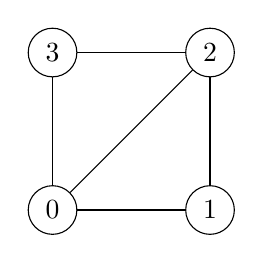
\begin{tikzpicture}
\node[shape=circle,draw=black] (A) at (0,0) {0};
\node[shape=circle,draw=black] (B) at (2,0) {1};
\node[shape=circle,draw=black] (C) at (2,2) {2};
\node[shape=circle,draw=black] (D) at (0,2) {3};
\path [-] (A) edge node[left] {} (B);
\path [-] (B) edge node[left] {} (C);
\path [-] (C) edge node[left] {} (D);
\path [-] (D) edge node[left] {} (A);
\path [-] (A) edge node[left] {} (C);
\end{tikzpicture}\\
\end{center}
The adjacency matrix is:\\
\begin{equation*}
    \begin{bmatrix}
    0 & 1 & 1 & 1\\
    1 & 0 & 1 & 0\\
    1 & 1 & 0 & 1\\
    1 & 0 & 1 & 0
    \end{bmatrix}
\end{equation*}
\textbf{Adjacency matrix for directed graphs}: A $n \times n$ matrix $A$ where $A_{ij} = 1$ if there is an edge from $i$ to $j$, and $A_{ij} = 0$ otherwise.\\
examples of adjacency matrices for directed graphs:\\
Given the following graph:\\
\begin{center}
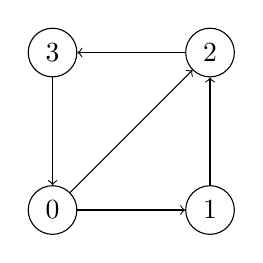
\begin{tikzpicture}
\node[shape=circle,draw=black] (A) at (0,0) {0};
\node[shape=circle,draw=black] (B) at (2,0) {1};
\node[shape=circle,draw=black] (C) at (2,2) {2};
\node[shape=circle,draw=black] (D) at (0,2) {3};
\path [->] (A) edge node[left] {} (B);
\path [->] (B) edge node[left] {} (C);
\path [->] (C) edge node[left] {} (D);
\path [->] (D) edge node[left] {} (A);
\path [->] (A) edge node[left] {} (C);
\end{tikzpicture}\\
\end{center}
The adjacency matrix is:\\
\begin{equation*}
    \begin{bmatrix}
    0 & 1 & 0 & 0\\
    0 & 0 & 1 & 0\\
    0 & 0 & 0 & 1\\
    1 & 0 & 0 & 0
    \end{bmatrix}
\end{equation*}
\textbf{Adjacency list}: A list of lists, where the $i$th list contains the neighbours of vertex $i$.\\
Given the following graph:\\
\begin{center}
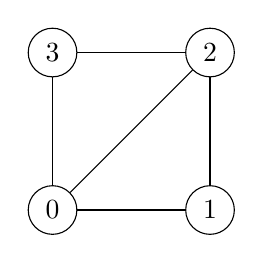
\begin{tikzpicture}
\centering
\node[shape=circle,draw=black] (A) at (0,0) {0};
\node[shape=circle,draw=black] (B) at (2,0) {1};
\node[shape=circle,draw=black] (C) at (2,2) {2};
\node[shape=circle,draw=black] (D) at (0,2) {3};
\path [-] (A) edge node[left] {} (B);
\path [-] (B) edge node[left] {} (C);
\path [-] (C) edge node[left] {} (D);
\path [-] (D) edge node[left] {} (A);
\path [-] (A) edge node[left] {} (C);
\end{tikzpicture}\\
\end{center}
The adjacency list is:\\
\begin{equation*}
    \begin{bmatrix}
    1 & 2 & 3\\
    0 & 2\\
    0 & 1 & 3\\
    0 & 2
    \end{bmatrix}
\end{equation*}
\textbf{Adjacency list for directed graphs}: A list of lists, where the $i$th list contains the neighbours of vertex $i$.\\
Given the following graph:\\
\begin{center}
    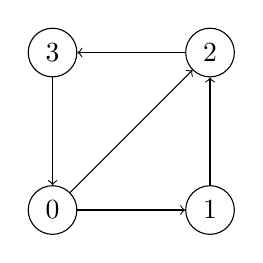
\begin{tikzpicture}
\centering
\node[shape=circle,draw=black] (A) at (0,0) {0};
\node[shape=circle,draw=black] (B) at (2,0) {1};
\node[shape=circle,draw=black] (C) at (2,2) {2};
\node[shape=circle,draw=black] (D) at (0,2) {3};
\path [->] (A) edge node[left] {} (B);
\path [->] (B) edge node[left] {} (C);
\path [->] (C) edge node[left] {} (D);
\path [->] (D) edge node[left] {} (A);
\path [->] (A) edge node[left] {} (C);
\end{tikzpicture}\\
\end{center}

The adjacency list is:\\
\begin{equation*}
    \begin{bmatrix}
    1 & 2\\
    2\\
    3\\
    0
    \end{bmatrix}
\end{equation*}
\textbf{Adjacency matrix vs adjacency list}:\\
\begin{table}[H]
\centering
\begin{tabular}{|c|c|}
\hline
Adjacency matrix & Adjacency list\\
\hline
$O(1)$ to check if there is an edge between $i$ and $j$ & $O(min(deg(i),deg(j)))$ to check if there is an edge between $i$ and $j$\\
\hline
$O(n)$ to find the neighbours of $i$ & $O(deg(j))$ to find the neighbours of $i$\\
\hline
$O(n^2)$ space & $O(n+m)$ space\\
\hline
\end{tabular}
\end{table}

\section{Depth-first search}
\textbf{Depth-first search}: A graph search algorithm that explores the neighbours of a vertex before exploring the neighbours of its neighbours.\\
example of depth-first search:\\
\begin{center}
    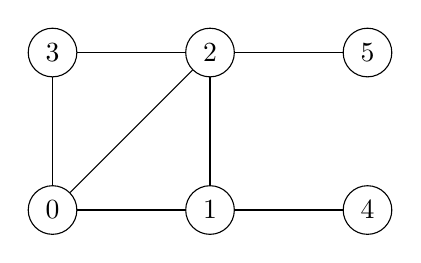
\begin{tikzpicture}
\centering
\node[shape=circle,draw=black] (A) at (0,0) {0};
\node[shape=circle,draw=black] (B) at (2,0) {1};
\node[shape=circle,draw=black] (C) at (2,2) {2};
\node[shape=circle,draw=black] (D) at (0,2) {3};
\node[shape=circle,draw=black] (E) at (4,0) {4};
\node[shape=circle,draw=black] (F) at (4,2) {5};
\path [-] (A) edge node[left] {} (B);
\path [-] (B) edge node[left] {} (C);
\path [-] (C) edge node[left] {} (D);
\path [-] (D) edge node[left] {} (A);
\path [-] (A) edge node[left] {} (C);
\path [-] (E) edge node[left] {} (B);
\path [-] (F) edge node[left] {} (C);
\end{tikzpicture}\\
\end{center}
The depth-first search sequence is:\\
\begin{equation*}
    0,1,2,3,5,4
\end{equation*}
\textbf{Depth-first search algorithm}:\\
\begin{algorithm}[H]
\caption{Depth-first search algorithm}
\begin{algorithmic}[1]
\Procedure{DFS}{$G,v$}
\For {$e \in V$}
\If {$e$ is unexplored}
\State $u$ = head of $e$
\If {$u$ is unexplored}
\State $e$ is a tree edge
\State \Call{DFS}{$G,u$}
\Else
\State $e$ is a back edge
\EndIf
\EndIf
\EndFor
\EndProcedure
\end{algorithmic}
\end{algorithm}
\textbf{Running time of depth-first search}: $O(n+m)$\\


\section{Breadth-first search}
\textbf{Breadth-first search}: A graph search algorithm that explores the neighbours of a vertex before exploring the neighbours of its neighbours.\\
exaqmple of breadth-first search:\\
\begin{center}
    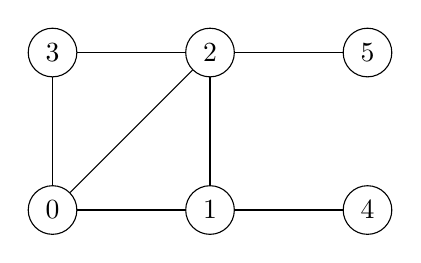
\begin{tikzpicture}
\centering
\node[shape=circle,draw=black] (A) at (0,0) {0};
\node[shape=circle,draw=black] (B) at (2,0) {1};
\node[shape=circle,draw=black] (C) at (2,2) {2};
\node[shape=circle,draw=black] (D) at (0,2) {3};
\node[shape=circle,draw=black] (E) at (4,0) {4};
\node[shape=circle,draw=black] (F) at (4,2) {5};
\path [-] (A) edge node[left] {} (B);
\path [-] (B) edge node[left] {} (C);
\path [-] (C) edge node[left] {} (D);
\path [-] (D) edge node[left] {} (A);
\path [-] (A) edge node[left] {} (C);
\path [-] (E) edge node[left] {} (B);
\path [-] (F) edge node[left] {} (C);
\end{tikzpicture}\\
\end{center}
The breadth-first search sequence starting from vertex 0 is 0, 1, 2, 3, 4, 5.\\
\textbf{Breadth-first search algorithm}:\\
\begin{algorithm}[H]
\caption{Breadth-first search algorithm}
\begin{algorithmic}[1]
\Procedure{BFS}{$G,s$}
\State initial empty list $L$
\State $L \gets {s}$
\State $i \gets 0$
\While{$L[i] \neq \emptyset$}
\State $L_{i+1} \gets empty list$
\For{$v \in L[i]$}
\For{edges $(e)$ incident to $v$}
\If{$e$ is unexplored}
\State $w \gets$ the other end of $e$
\If {$w$ is unexplored}
\State label $e$ as a tree edge
\State add $w$ to $L_{i+1}$
\Else
\State label $e$ as a cross edge
\EndIf
\EndIf
\EndFor
\EndFor
\State $i \gets i+1$
\EndWhile
\EndProcedure
\end{algorithmic}
\end{algorithm}
\textbf{Running time of breadth-first search}: $O(n+m)$\\


\section{Strong Connectivity}
\textbf{Directed graph}: A graph where the edges have a direction.\\
Examples:\\
\begin{center}
    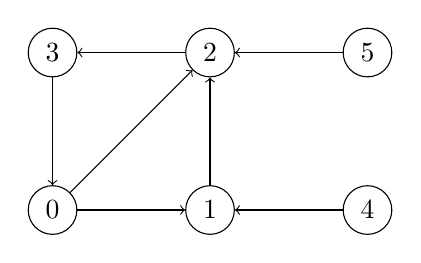
\begin{tikzpicture}
\centering
\node[shape=circle,draw=black] (A) at (0,0) {0};
\node[shape=circle,draw=black] (B) at (2,0) {1};
\node[shape=circle,draw=black] (C) at (2,2) {2};
\node[shape=circle,draw=black] (D) at (0,2) {3};
\node[shape=circle,draw=black] (E) at (4,0) {4};
\node[shape=circle,draw=black] (F) at (4,2) {5};
\path [->] (A) edge node[left] {} (B);
\path [->] (B) edge node[left] {} (C);
\path [->] (C) edge node[left] {} (D);
\path [->] (D) edge node[left] {} (A);
\path [->] (A) edge node[left] {} (C);
\path [->] (E) edge node[left] {} (B);
\path [->] (F) edge node[left] {} (C);
\end{tikzpicture}\\
\end{center}
\noindent
\textbf{DFS and BFS on directed graphs}:\\
Very similar to undirected graphs, except that we only consider edges that go out of a vertex.\\
Running time is $O(n+m)$\\
For example graph above the DFS sequence is 0, 1, 2, 3.\\
The BFS sequence is 0, 1, 2, 3.\\
\subsection{Connectivity}
\textbf{Weak connectivity}:If we ignore the direction for all edges, there would be a pah from any vertex to any other vertex.\\
\textbf{Strong Connectivity}:For every two nodes $u$ and $v$, there is a path from $u$ to $v$ and a path from $v$ to $u$.\\

\subsection{Mutual Reachability}
Two nodes $u$ and $v$ are mutually reachable if there is a path from $u$ to $v$ and a path from $v$ to $u$.\\
\textbf{Strong connectivity}:For every pair of nodes $u$ and $v$, these two nodes are mutually reachable.\\
\textbf{Transitivity}:If $u$ is mutually reachable with $v$ and $v$ is mutually reachable with $w$, then $u$ is mutually reachable with $w$.\\
\\


\subsection{Testing strong connectivity}
\begin{algorithm}[H]
\caption{Testing strong connectivity}
\begin{algorithmic}[1]
\Procedure{TestStrongConnectivity}{$G$}
\State define $G^R$ to be the graph with the same vertices as $G$ but with all edges reversed
\State Select a node $s$ in $G$
\State BFS($G,s$),BFS($G^R,s$)
\For{each node $v$}
\If{$v$ is unexplored in either BFS}
\State \Return False
\EndIf
\EndFor
\State \Return True
\EndProcedure
\end{algorithmic}
\end{algorithm}

\section{Testing bipartiteness}
\textbf{Bipartite graph}: A graph $G=(V,E)$ is bipartite if any only if the vertices can be partitioned into two sets $V_1$ and $V_2$ such that every edge has one end in $V_1$ and the other end in $V_2$.\\
A Graph $G=(V,E)$ is bipartite if and only if it has no odd cycles.(odd cycle: a cycle with odd number of edges)\\
\noindent
\textbf{Testing bipartiteness}:\\
Given a graph $G=(V,E)$, we want to test if $G$ is bipartite.\\
Given a graph $G=(V,E)$, decide if it is 2-colourable.\\
Given a graph $G=(V,E)$, decide if it has an odd cycle.\\
\noindent
\textbf{Colouring the nodes}
It is quite familiar with BFS:\\
\begin{algorithm}[H]
\caption{Colouring the nodes}
\begin{algorithmic}[1]
\Procedure{Colouring}{$G,s$}
\State initial empty list $L$
\State initial empty list $C$
\State $L \gets {s}$
\State $C[s] \gets red$
\State $i \gets 0$
\While{$L[i] \neq \emptyset$}
\State $L_{i+1} \gets empty list$
\For{$v \in L[i]$}
\For{edges $(e)$ incident to $v$}
\If{$e$ is unexplored}
\State $w \gets$ the other end of $e$
\If {$w$ is unexplored}
\State label $e$ as a tree edge
\State add $w$ to $L_{i+1}$
\If {$i+1$ is odd}
\State $C[w] \gets green$
\Else 
\State $C[w] \gets red$
\EndIf
\Else
\State label $e$ as a cross edge
\If{$C[v] = C[w]$}
\State \Return False
\EndIf
\EndIf
\EndIf
\EndFor
\EndFor
\State $i \gets i+1$
\EndWhile
\For {$e(v,w) \in G$}
\If {$C[v] = C[w]$}
\State \Return False
\EndIf
\EndFor
\State \Return True
\EndProcedure
\end{algorithmic}
\end{algorithm}
\noindent
\textbf{Running time of colouring the nodes}: $O(n+m)$\\
\textbf{Correctness of colouring the nodes}:\\
Proof by contradiction.\\
Suppose that $G$ is not bipartite.\\
Then $G$ has an odd cycle.\\
Suppose to the contrary that the algorithm return True.\\
That means that the algorithm did not detect the odd cycle.\\

\section{DAGs and Topological Ordering}
\textbf{DAG}: A directed acyclic graph (DAG) is a directed graph with no directed cycles.\\
examples of DAGs:\\
\begin{center}
    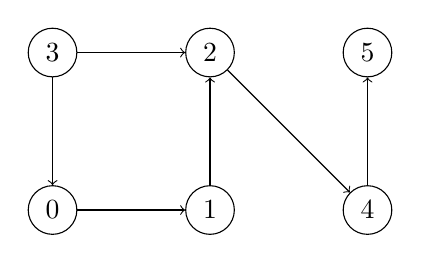
\begin{tikzpicture}
\centering
\node[shape=circle,draw=black] (A) at (0,0) {0};
\node[shape=circle,draw=black] (B) at (2,0) {1};
\node[shape=circle,draw=black] (C) at (2,2) {2};
\node[shape=circle,draw=black] (D) at (0,2) {3};
\node[shape=circle,draw=black] (E) at (4,0) {4};
\node[shape=circle,draw=black] (F) at (4,2) {5};
\path [->] (A) edge node[left] {} (B);
\path [->] (B) edge node[left] {} (C);
\path [->] (C) edge node[left] {} (E);
\path [->] (D) edge node[left] {} (A);
\path [->] (D) edge node[left] {} (C);
\path [->] (E) edge node[left] {} (F);
\end{tikzpicture}\\
\end{center}
\noindent
\textbf{Topological ordering}:Given a graph$G=(V,E)$, a topological ordering of $G$ is an ordering of the nodes $u_1,u_2,\dots,u_n$ such that for every edge $(u_i,u_j)$, we have $i<j$.\\
Intutively, a topological ordering is an ordering of the nodes such that every edge goes from left to right.\\
example of topological ordering based on given graph above:\\
\begin{equation*}
    3,0,1,2,4,5
\end{equation*}
\noindent
\textbf{Topological ordering implies DAG}:\\
\begin{itemize}
    \item If $G$ has a topological ordering, then $G$ is a DAG.
    \item Suppose by contradiction that $G$ has a topological ordering $u_1,u_2,\dots,u_n$ but $G$ also has a cycle $C$.
    \item Let $u_j$ be the smallest element of $C$ in the topological ordering.
    \item Let $u_i$ be its predecessor in $C$.
    \item $u_i$ must appear before $u_j$ in the topological ordering.
    \item This contradicts the fact that $u_j$ is the smallest element of $C$ in the topological ordering.
\end{itemize}

\noindent
\textbf{DAG implies topological ordering}:\\
Proof by induction:
Base case: If $G$ has one or two nodes, then $G$ has a topological ordering.\\
Induction steps: Assume that a DAG up to $k$ nodes has a topological ordering(induction hypothesis). we will prove that a DAG with $k+1$ nodes has a topological ordering.
\begin{itemize}
    \item By our lemma, there is at least one source node in $G$, and let $u$ be the node.
    \item Put $u$ at the beginning of the topological ordering.
    \item Consider the graph $G'$, obtained by $G$ by removing $u$ and its incident edges.
    \item $G'$ is a DAG with $k$ nodes.
    \item It has a topological ordering $u_1,u_2,\dots,u_k$ by the induction hypothesis.
    \item Append this ordering to $u$ to get a topological ordering of $G$.
\end{itemize}
\noindent
Here is the algorithm:\\
\begin{algorithm}[H]
\caption{Topological Sorting}
\begin{algorithmic}[1]
\Procedure{TopologicalSorting}{$G$}
\State find a source vertex $u$
\State set $u$ as the first element of the topological ordering
\State $G' \gets G$ with $u$ and its incident edges removed
\State $L \gets$ \Call{TopologicalSorting}{$G'$}
\State append $L$ to $u$
\EndProcedure
\end{algorithmic}
\end{algorithm}
\noindent
Running time of the algorithm is $O(n^2)$\\
\textbf{Modified Topological Sorting}:\\
Running time of the algorithm is $O(n+m)$\\
\begin{algorithm}[H]
\caption{Modified Topological Sorting}
\begin{algorithmic}[1]
\Procedure{ModifiedTopologicalSorting}{$G$}
\State $L \gets empty list$
\State $S \gets$ set of all source vertices
\While{$S \neq \emptyset$}
\State remove a vertex $u$ from $S$
\State append $u$ to $L$
\For{each edge $(u,v)$}
\State remove edge $(u,v)$ from $G$
\If{$v$ is a source vertex}
\State add $v$ to $S$
\EndIf
\EndFor
\EndWhile
\If{$G$ has edges}
\State \Return $G$ has a cycle
\Else
\State \Return $L$
\EndIf
\EndProcedure
\end{algorithmic}
\end{algorithm}

\section{Finding strongly connected components}
\textbf{connected components}: A connected component of an undirected graph is subgraph of the graph where any two nodes are connected by a path.\\
\textbf{strongly connected components}: A strongly connected component of a directed graph is a subgraph of the graph where any two nodes are mutually reachable.(mutually reachable: there is a path from $u$ to $v$ and a path from $v$ to $u$)\\
\textbf{Finding strongly connected components}:\\
\textbf{Kosaraju's algorithm}:\\
\begin{algorithm}[H]
\caption{Kosaraju's algorithm}
\begin{algorithmic}[1]
\Procedure{Kosaraju}{$G$}
\State Initialise stack $S$
\State Select a arbitrary node $s$
\State DFS\_tree=DFS($G,s$)
\State $S \gets$ nodes in DFS\_tree
\State $G^R \gets$ nodes in order of $S$
\State DFS($G^R,s$)
\State \Return the nodes in the DFS tree
\EndProcedure
\end{algorithmic}
\end{algorithm}
\noindent
\textbf{Running time of Kosaraju's algorithm}: $O(n+m)$\\
\textbf{Correctness of Kosaraju's algorithm}:
\begin{itemize}
    \item Define a meta-graph of $G$, called $G^{SCC}=(V^{SCC},E^{SCC})$.
    \item Supposed that $G$ has strongly connected components (SCCs) $C_1,C_2,\dots,C_k$, for some $k$.
    \item $V^{SCC} = \{C_1,C_2,\dots,C_k\}$ contains some of the SCCs of $G$.
    \item There is an edge $(C_i,C_j)$ in $E^{SCC}$ if $G$ contains a directed edge ($x,y$) such that $x \in C_i$ and $y \in C_j$, crossing different components.
\end{itemize}
\noindent
Examples:
\begin{center}
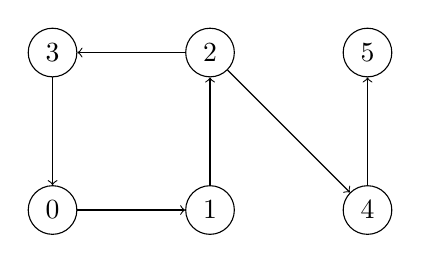
\begin{tikzpicture}
\centering
\node[shape=circle,draw=black] (A) at (0,0) {0};
\node[shape=circle,draw=black] (B) at (2,0) {1};
\node[shape=circle,draw=black] (C) at (2,2) {2};
\node[shape=circle,draw=black] (D) at (0,2) {3};
\node[shape=circle,draw=black] (E) at (4,0) {4};
\node[shape=circle,draw=black] (F) at (4,2) {5};
\path [->] (A) edge node[left] {} (B);
\path [->] (B) edge node[left] {} (C);
\path [->] (C) edge node[left] {} (E);
\path [->] (D) edge node[left] {} (A);
\path [->] (C) edge node[left] {} (D);
\path [->] (E) edge node[left] {} (F);
\end{tikzpicture}\\
\end{center}
\noindent
The SCCs are $\{0,1,2,3\}$ and $\{4,5\}$.\\
\noindent
The meta-graph is:\\
\begin{center}
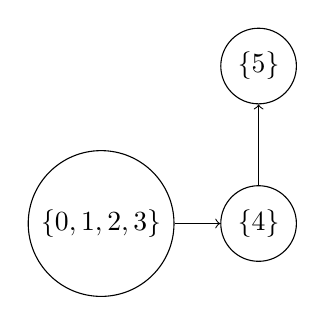
\begin{tikzpicture}
\centering
\node[shape=circle,draw=black] (A) at (0,0) {$\{0,1,2,3\}$};
\node[shape=circle,draw=black] (B) at (2,0) {$\{4\}$};
\node[shape=circle,draw=black] (C) at (2,2) {$\{5\}$};
\path [->] (A) edge node[left] {} (B);
\path [->] (B) edge node[left] {} (C);
\end{tikzpicture}\\
\end{center}
\noindent


\chapter{Greedy Algorithms}
\textbf{The greedy approach}:
\begin{itemize}
    \item The goal is to find a global solution to a problem.
    \item The solution will be built up in small consecutive steps.
    \item For each step, we choose the best option available to us at that moment.
\end{itemize}
\section{Interval Scheduling}
\textbf{Interval Scheduling}:\\
A set of requests$R=\{1,2,\dots,n\}$.
\begin{itemize}
    \item Each request $i$ has a start time $s_i$ and a finish time $f_i$.
    \item Alternative view: every request is an interval $[s_i,f_i]$.
\end{itemize}
Two requests $i$ and $j$ are compatible if $[s_i,f_i]$ and $[s_j,f_j]$ do not overlap.\\
\textbf{Goal}: Find a maximum-size subset of compatible requests.\\
\textbf{Example}:\\
\begin{figure}[H]
    \centering
    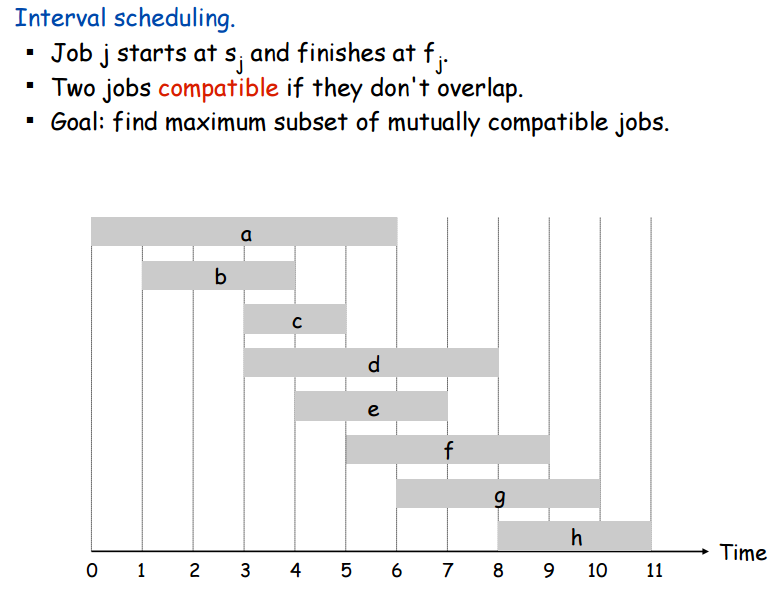
\includegraphics[width=0.65\linewidth]{figures/scheduling.png}
    \caption{Interval Scheduling}
    \label{fig:my_label}
\end{figure}
\noindent
\textbf{Interval Scheduling Algorithm}:
\begin{algorithm}[H]
\caption{Interval Scheduling Algorithm}
\begin{algorithmic}[1]
\Procedure{IntervalScheduling}{$[s_1,f_1],[s_2,f_2],\dots,[s_n,f_n]$}
\State $R$ is the set of requests
\State $A \gets \emptyset$
\While{$R \neq \emptyset$}
\State select a request $i$ in $R$ with the smallest finishing time
\State add $i$ to $A$
\State remove all requests from $R$ that are incompatible with $i$
\EndWhile
\State \Return $A$
\EndProcedure
\end{algorithmic}
\end{algorithm}
\noindent
\textbf{Running time of Interval Scheduling Algorithm}: $O(n\log n)$\\
\textbf{Correctness of Interval Scheduling Algorithm}:
Since the algorithm always selects the request with the smallest finishing time, it is clear that the algorithm will always select a compatible request.\\
\textbf{Arguing optimality}:\\


\section{Minimum Spanning Trees}
Consider a connected graph $G=(V,E)$, such that each edge $e=(v,w)$ of $E$, there is an associated cost $c_e$.\\
\textbf{Goal}: Find a spanning tree $T$ of $E$ so that the graph $G'=(V,T)$ has minimum cost.\\
\textbf{Example}:\\
\begin{center}
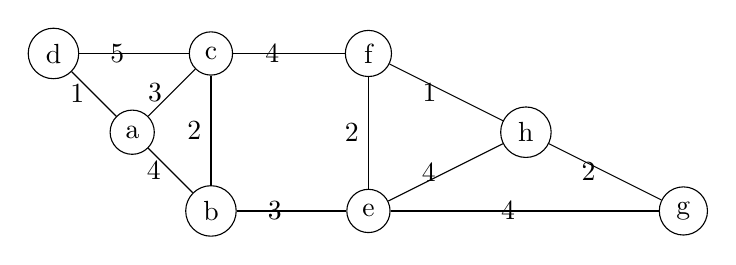
\begin{tikzpicture}
\centering
\node[shape=circle,draw=black] (A) at (1,1) {a};
\node[shape=circle,draw=black] (B) at (2,0) {b};
\node[shape=circle,draw=black] (C) at (2,2) {c};
\node[shape=circle,draw=black] (D) at (0,2) {d};
\node[shape=circle,draw=black] (E) at (4,0) {e};
\node[shape=circle,draw=black] (F) at (4,2) {f};
\node[shape=circle,draw=black] (G) at (8,0) {g};
\node[shape=circle,draw=black] (H) at (6,1) {h};
\path [-] (A) edge node[left] {4} (B);
\path [-] (A) edge node[left] {3} (C);
\path [-] (A) edge node[left] {1} (D);
\path [-] (B) edge node[left] {2} (C);
\path [-] (B) edge node[left] {3} (E);
\path [-] (C) edge node[left] {5} (D);
\path [-] (C) edge node[left] {4} (F);
\path [-] (E) edge node[left] {4} (G);
\path [-] (E) edge node[left] {2} (F);
\path [-] (F) edge node[left] {1} (H);
\path [-] (G) edge node[left] {2} (H);
\path [-] (E) edge node[left] {4} (H);
\end{tikzpicture}\\
\end{center}

\textbf{Greedy approach 1}:\\
\begin{itemize}
    \item Start with an empty set of edges $T$.
    \item Repeat until $T$ forms a spanning tree:
    \begin{itemize}
        \item Select an edge $e$ of minimum cost.
        \item If $T \cup \{e\}$ does not contain a cycle, then add $e$ to $T$.
    \end{itemize}
\end{itemize}
\textbf{krukals algorithm}:
\begin{algorithm}[H]
\caption{Krukals algorithm}
\begin{algorithmic}[1]
\Procedure{Krukals}{$G$}
\State $T \gets \emptyset$
\While{$T$ is not a spanning tree}
\State select an edge $e$ of minimum cost
\If{$T \cup \{e\}$ does not contain a cycle}
\State add $e$ to $T$
\EndIf
\EndWhile
\State \Return $T$
\EndProcedure
\end{algorithmic}
\end{algorithm}

\noindent
\textbf{Running time of Krukals algorithm}: $O(m\log n)$\\
\textbf{Greedy approach 2}:
\begin{itemize}
    \item Start with an empty set of edges $T$.
    \item Start with a node $s$.
    \begin{itemize}
        \item Add an edge $e=(s,v)$ of minimum cost to $T$.
    \end{itemize}
    \item Repeat until $T$ forms a spanning tree:
\end{itemize}
\textbf{Prims algorithm}:
\begin{algorithm}[H]
\caption{Prims algorithm}
\begin{algorithmic}[1]
\Procedure{Prims}{$G$}
\State $T \gets \emptyset$
\State $s \gets$ an arbitrary node
\While{$T$ is not a spanning tree}
\State add an edge $e=(s,v)$ of minimum cost to $T$
\State $s \gets v$
\EndWhile
\State \Return $T$
\EndProcedure
\end{algorithmic}
\end{algorithm}
\noindent
\textbf{Running time of Prims algorithm}: $O(m\log n)$\\
\textbf{minimum spanning tree of example graph}:\\
the minimum spanning tree sequence is $d,a,c,b,e,f,h,g$.\\
\noindent

\textbf{Greedy approach 3}:\\
\begin{itemize}
    \item Start with the full graph $G=(V,E)$.
    \item Delete an edge from $G$
    \begin{itemize}
        \item the edge of maximum cost
    \end{itemize}
    \item Repeat until $G$ forms a spanning tree:
\end{itemize}
\textbf{Reverse-delete algorithm}:
\begin{algorithm}[H]
\caption{Reverse-delete algorithm}
\begin{algorithmic}[1]
\Procedure{ReverseDelete}{$G$}
\State $T \gets G$
\While{$T$ is not a spanning tree}
\State delete an edge $e$ of maximum cost from $T$
\EndWhile
\State \Return $T$
\EndProcedure
\end{algorithmic}
\end{algorithm}
\noindent
For when two edges have the same cost, use distinct labels to distinguish them.\\

\noindent
\textbf{Optimal with Priorty Queue}:\\
Add PQ to Prim's algorithm.\\
\begin{algorithm}[H]
\caption{Optimal with Priorty Queue}
\begin{algorithmic}[1]
\Procedure{Optimal}{$G$}
\State $T \gets \emptyset$
\State $s \gets$ an arbitrary node
\State $PQ \gets$ empty priority queue
\For{each node $v$}
\State add $v$ to $PQ$ with key $\infty$
\EndFor
\State decrease key of $s$ to 0
\While{$PQ$ is not empty}
\State $v \gets$ node with minimum key in $PQ$
\State add an edge $e=(s,v)$ of minimum cost to $T$
\State $s \gets v$
\For{each edge $e=(v,w)$ incident to $v$}
\If{$w$ is in $PQ$}
\State decrease key of $w$ to $c_e$
\EndIf
\EndFor
\EndWhile
\State \Return $T$
\EndProcedure
\end{algorithmic}
\end{algorithm}
\noindent
\textbf{Running time of Optimal with Priorty Queue}: $O(m\log n)$\\

\section{Clustering}
\begin{itemize}
    \item a collection of $n$ objects
    \item they have different degrees of similarity
    \item we want to organise them into coherent groups
    \item there is a notion of distance between objects
\end{itemize}
\noindent
\textbf{Definition}:
\begin{itemize}
    \item Given a set $U$ of $n$ elements, a $k-$clustering of $U$ is a partition of $U$ into non-empty subsets $C_1,C_2,\dots,C_k$.
    \item The spacing of a $k-$clustering is the minimum distance between any pair of points in different clusters.
\end{itemize}
\textbf{Goal}:Among all possible $k-$clusterings, find one with minimum spacing.\\
\textbf{Example}:\\
\begin{center}
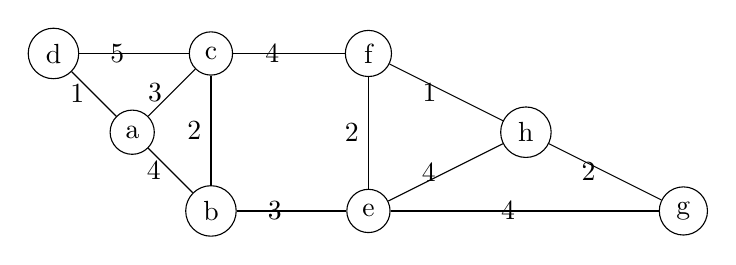
\begin{tikzpicture}
\centering
\node[shape=circle,draw=black] (A) at (1,1) {a};
\node[shape=circle,draw=black] (B) at (2,0) {b};
\node[shape=circle,draw=black] (C) at (2,2) {c};
\node[shape=circle,draw=black] (D) at (0,2) {d};
\node[shape=circle,draw=black] (E) at (4,0) {e};
\node[shape=circle,draw=black] (F) at (4,2) {f};
\node[shape=circle,draw=black] (G) at (8,0) {g};
\node[shape=circle,draw=black] (H) at (6,1) {h};
\path [-] (A) edge node[left] {4} (B);
\path [-] (A) edge node[left] {3} (C);
\path [-] (A) edge node[left] {1} (D);
\path [-] (B) edge node[left] {2} (C);
\path [-] (B) edge node[left] {3} (E);
\path [-] (C) edge node[left] {5} (D);
\path [-] (C) edge node[left] {4} (F);
\path [-] (E) edge node[left] {4} (G);
\path [-] (E) edge node[left] {2} (F);
\path [-] (F) edge node[left] {1} (H);
\path [-] (G) edge node[left] {2} (H);
\path [-] (E) edge node[left] {4} (H);
\end{tikzpicture}\\
\end{center}
\textbf{Greedy approach}:\\
\begin{itemize}
    \item Pick two objects $p_i$ and $p_j$ with minimum distance $d(p_i,p_j)$.
    \item Connect them with an edge $e=(p_i,p_j)$.
    \item Continue like this until we have $k$ clusters.
    \item If the edge $e$ under consideration connects two object $p_i$ and $p_j$ already in the same cluster, then discard $e$.
\end{itemize}
\textbf{kruskals algorithm}:
\begin{algorithm}[H]
\caption{kruskals algorithm for clustering}
\begin{algorithmic}[1]
    \Require A graph $G = (V,E)$
    \Ensure A minimum spanning tree of $G$ with $k$ clusters
    
    \Procedure{Kruskal}{$G,k$}
      \State $T \gets \emptyset$
      \State $C \gets \{ \{v\} \mid v \in V \}$ \Comment{Initial clusters}
      \State Sort edges in $E$ in increasing order of weight
      \For{$\{u,v\} \in E$}
        \If{$C$ contains $k$ clusters}
          \State \textbf{break}
        \EndIf
        \If{clusters containing $u$ and $v$ are different in $C$}
          \State $T \gets T \cup \{\{u,v\}\}$
          \State merge clusters containing $u$ and $v$ in $C$
        \EndIf
      \EndFor
      \State \textbf{return} $T$
    \EndProcedure
\end{algorithmic}
\end{algorithm}
\noindent
For Given example, the result of divide them into 3 clusters is:\\
\begin{equation*}
    \{a,b,c,d\},\{e,f,h\},\{g\}
\end{equation*}
\noindent

\chapter{Dynamic Programming}
\textbf{The paradigm of dynamic programming}:
Given a problem $P$, define a sequence of subproblems, with the following properties:
\begin{itemize}
    \item The subproblems are ordered from the simplest to the largest
    \item The largest problem is our original problem $P$
    \item The optimal solution of a subproblem can be structured from the optimal solutions of smaller subproblems.
\end{itemize}
Solve the subproblems from the smallest to the largest. When you solve a subproblem, store the solution and use it to solve larger subproblems.\\
\section{Weighted Interval Scheduling}
\begin{itemize}
    \item A set of requests $R=\{1,2,\dots,n\}$.
    \begin{itemize}
        \item Request $i$ has a start time $s_i$ and a finish time $f_i$, and a value $v_i$.
        \item Alternative view: every request is an interval $[s_i,f_i]$ associated with a value $v_i$.
    \end{itemize}
    \item Two requests $i$ and $j$ are compatible if $[s_i,f_i]$ and $[s_j,f_j]$ do not overlap.
\end{itemize}
\textbf{build up a solution}:
\begin{enumerate}
    \item let $O$ the optimal solution
    \item $O$ contains an optimal solution $O'$ of the subproblem $R'=\{1,2,\dots,i-1\}$
    \item in order to find $O$, it suffices to look at smaller problems and find $O(1,2,\dots,j)$ for some $j$
    \item Let $O_j$ be a shorthand for $O(1,2,\dots,j)$ and let $OPT(j)$ be its total value.
    \item Define $OPT(0)=0$
    \item Then $O=O_n$ with value $OPT(n)$
    \item $OPT(j)$ can be computed from $OPT(j-1)$
    \item $OPT(j)=\max\{OPT_{p_j}+v_j,OPT(j-1)\}$
\end{enumerate}

\begin{algorithm}[H]
\caption{ComputeOPT}
\begin{algorithmic}[1]
    \Procedure{ComputeOPT}{$j$}
        \If{$j=0$}
            \State \textbf{return} $0$
        \Else
            \State \textbf{return} $\max\{\textsc{ComputeOPT}(p_j)+v(j),\textsc{ComputeOPT}(j-1)\}$
        \EndIf
    \EndProcedure
\end{algorithmic}
\end{algorithm}
\noindent
\textbf{Correctness}:
ComputeOPT(j) correctly computes $OPT(j)$ for all $j=0,1,\dots,n$.\\
Proof by induction:\\
\textbf{Base case}: $OPT(0)=0$ by definition.\\
\textbf{Inductive step}: Assume that it is true for all $i<j$.(Induction hypothesis)\\
return $\max\{\textsc{ComputeOPT}(p_j)+v(j),\textsc{ComputeOPT}(j-1)\}$\\
\noindent
\textbf{Running time}: $\Omega(2^n)$\\
\textbf{Memoization}:
\begin{itemize}
    \item Compute ComputeOPT(j) for all $j=0,1,\dots,n$.
    \item Store it in an accessible place to use again later.
    \item Keep an array $M[0,\dots,n]$.
    \begin{itemize}
        \item initially $M[j]=\textsc{empty}$ for all $j=0,1,\dots,n$.
        \item when ComputeOPT(j) is called, $M[j]=$ ComputeOPT(j).
    \end{itemize}
\end{itemize}
\begin{algorithm}[H]
\caption{M-ComputeOPT}
\begin{algorithmic}
    \Procedure{M-ComputeOPT}{$j$}
        \If {$j=0$}
            \State \textbf{return} $0$
        \ElsIf {$M[j]$ is not empty}
            \State \textbf{return} $M[j]$
        \Else
            \State $M[j] \gets \max\{\textsc{M-ComputeOPT}(p_j)+v(j),\textsc{M-ComputeOPT}(j-1)\}$
            \State \textbf{return} $M[j]$
        \EndIf
    \EndProcedure
\end{algorithmic}
\end{algorithm}
\noindent
\textbf{Running time}: $O(n \log n)$\\
\begin{algorithm}[H]
\caption{Find-Solution}
\begin{algorithmic}
    \Procedure{Find-Solution}{$j$}
        \If {$j=0$}
            \State \textbf{return} $\emptyset$
        \Else 
            \If $v(j)+\textsc{M-ComputeOPT}(p_j)>\textsc{M-ComputeOPT}(j-1)$
                \State \textbf{return} $\{j\} \cup \textsc{Find-Solution}(p_j)$
            \Else
                \State \textbf{return} $\textsc{Find-Solution}(j-1)$
            \EndIf
        \EndIf
    \EndProcedure
\end{algorithmic}
\end{algorithm}
\noindent
\clearpage
\noindent
\textbf{Dynamic Programming vs Divide and Conquer}:
\begin{multicols}{2}
\noindent
\textbf{Dynamic Programming}:
\begin{itemize}
    \item DP is an optimisation techniques and is only applicable to problems that have optimal substructure.
    \item DP splits the problem into parts, finds solutions to the parts and joins them.(The parts are not significantly smaller than the original problem and are overlapping.)
    \item In DP, the subproblems dependency can be represented by a directed acyclic graph.
\end{itemize}
\columnbreak
\textbf{Divide and Conquer}:
\begin{itemize}
    \item DC is not normally used for optimisation problems.
    \item DC splits the problem into parts, finds solutions to the parts and joins them.(The parts are significantly smaller than the original problem and are non-overlapping.)
    \item In DC, the subproblems dependency can be represented by a tree.
\end{itemize}
\end{multicols}
\noindent
\section{Subset Sum}
\textbf{Problem Description}:
\begin{itemize}
    \item Given a set of $n$ items ${1,2,\dots,n}$
    \item Each item $i$ has a non-negative weight $w_i$.
    \item Given a bound $W$.
    \item \textbf{Goal}: select a subset $S$ of items such that $\sum_{i\in S}w_i\leq W$ and $\sum_{i\in S}w_i$ is maximised.
\end{itemize}
Dynamic Programming:
To find the optimal value of $OPT(n)$, we need
\begin{itemize}
    \item the optimal value of $OPT(n-1)$ if item $n$ is not selected.
    \item the optimal value of the solution on input {1,2,\dots,n-1} with weight bound $W-w_n$.
\end{itemize}
subproblems:
\begin{itemize}
    \item Assumptions:
    \begin{itemize}
        \item $W$ is an integer
        \item Every $w_i$ is an integer
    \end{itemize}
    \item subproblem for each $i=0,1,\dots,n$ and each integer $0 \leq w \leq W$.
    \item Let $OPT(i,w)$ be the optimal value of the solution on subset ${1,2,\dots,i}$ with weight bound $w$.
\end{itemize}
\begin{algorithm}[H]
\caption{SubsetSum}
\begin{algorithmic}
    \Procedure{SubsetSum}{$n,w$}
        \State Array $M[0,\dots,n,0,\dots,W]$
        \State $M[0,w]=0$ for each $w=0,1,\dots,W$
        \For {$i=1$ to $n$}
            \For {$w=0$ to $W$}
                \If {$w_i>w$}
                    \State $M[i,w]=M[i-1,w]$
                \Else
                    \State $M[i,w]=\max\{M[i-1,w],M[i-1,w-w_i]+w_i\}$
                \EndIf
            \EndFor
        \EndFor
        \State \textbf{return} $M[n,W]$
    \EndProcedure
\end{algorithmic}
\end{algorithm}
\noindent
\textbf{Running time}: $O(nW)$\\


\section{knapSack}
\textbf{Problem Description}:
\begin{itemize}
    \item Given a set of $n$ items ${1,2,\dots,n}$
    \item Each item $i$ has a non-negative weight $w_i$ and a non-negative value $v_i$.
    \item Given a bound $W$.
    \item \textbf{Goal}: select a subset $S$ of items such that $\sum_{i\in S}w_i\leq W$ and $\sum_{i\in S}v_i$ is maximised.
\end{itemize}
\textbf{the fractional knapsack problem}:
\begin{itemize}
    \item Given a set of $n$ items ${1,2,\dots,n}$
    \item Each item $i$ has a non-negative weight $w_i$ and a non-negative value $v_i$.
    \item Given a bound $W$.
    \item \textbf{Goal}: select a fraction $x_i$ of each item $i$ such that $\sum_{i\in S}w_ix_i\leq W$ and $\sum_{i\in S}v_ix_i$ is maximised.
\end{itemize}
\textbf{The 0/1 knapsack problem}:
Solution for 0/1 knapsack problem:
\begin{algorithm}
\caption{0/1 knapsack in dynamic programming}
\begin{algorithmic}
    \Procedure{0/1 knapsack}{$n,W$}
        \State Array $M[0,\dots,n,0,\dots,W]$
        \State $M[0,w]=0$ for each $w=0,1,\dots,W$
        \For {$i=1$ to $n$}
            \For {$w=0$ to $W$}
                \If {$w_i>w$}
                    \State $M[i,w]=M[i-1,w]$
                \Else
                    \State $M[i,w]=\max\{M[i-1,w],M[i-1,w-w_i]+v_i\}$
                \EndIf
            \EndFor
        \EndFor
        \State \textbf{return} $M[n,W]$
    \EndProcedure
\end{algorithmic}
\end{algorithm}

\chapter{Network Flow}
\section{Network Flow Definitions}
\textbf{Flow network}:
A flow network is a directed graph $G=(V,E)$ with the following properties:
\begin{itemize}
    \item Each edge $(u,v)\in E$ has a non-negative capacity $c_e$.
    \item There is a single source $s$ in $V$.
    \item There is a single sink $t$ in $V$.
    \item All other nodes in $V-\{s,t\}$ are called intermediate nodes.
\end{itemize}
example:
\begin{center}
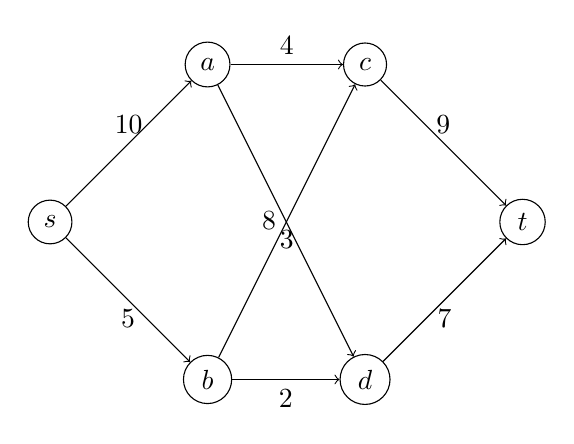
\begin{tikzpicture}
    \node[shape=circle,draw=black] (s) at (0,0) {$s$};
    \node[shape=circle,draw=black] (a) at (2,2) {$a$};
    \node[shape=circle,draw=black] (b) at (2,-2) {$b$};
    \node[shape=circle,draw=black] (c) at (4,2) {$c$};
    \node[shape=circle,draw=black] (d) at (4,-2) {$d$};
    \node[shape=circle,draw=black] (t) at (6,0) {$t$};
    \path [->] (s) edge node[above] {$10$} (a);
    \path [->] (s) edge node[below] {$5$} (b);
    \path [->] (a) edge node[above] {$4$} (c);
    \path [->] (a) edge node[left] {$8$} (d);
    \path [->] (b) edge node[below] {$3$} (c);
    \path [->] (b) edge node[below] {$2$} (d);
    \path [->] (c) edge node[above] {$9$} (t);
    \path [->] (d) edge node[below] {$7$} (t);
\end{tikzpicture}
\end{center}
\noindent
\textbf{Further definitions}:
\begin{itemize}
    \item The source $s$ has no incoming edges.
    \item The sink $t$ has no outgoing edges.
    \item There is at least one edge incident to each node.
    \item All capacities are integers.
\end{itemize}
\noindent
\textbf{Flow}:
An $(s-t)$ flow is a function $f:E \rightarrow \mathbb{R^+}$, mapping each edge $e$ to a non-negative real number $f(e)$.\\
A feasible flow must satisfy the following conditions:
\begin{itemize}
    \item Capacity: For each edge $e\in E$, $0 \leq f(e) \leq c_e$.
    \item Flow conservation: for each node $v\in V-\{s,t\}$, we have
    \begin{equation*}
        \sum_{e \:\text{into} \: v}f(e)=\sum_{e \: \text{out of}\: v}f(e)
    \end{equation*}
\end{itemize}
The source $s$ generates flow, and the sink $t$ absorbs flow.\\
Value of a flow $f$, denoted $val(f)$, is the total amount of flow generated by the source $s$:
\begin{equation*}
    v(f)=\sum_{e \: \text{out of}\: s}f(e)
\end{equation*}
Generally, define $f^{out}(v)$ and $f^{in}(v)$ for the flow going out of(resp. going into) node $v$.\\
Similarly, define $f^{out}(S)$ and $f^{in}(S)$ for sets of nodes $S$.\\

\noindent
\section{Maximum Flow Problem}
\textbf{The maximum flow problem}: Given a flow network $G=(V,E)$, find a flow of maximum possible value.\\
\textbf{algorithm for maximum flow}:\\
Idea: push flow forward on edges with leftover capacity, push flow backward on edges that are already carrying flow.\\
\noindent
\textbf{The residual graph $G_f$}:\\
The residual graph $G_f$ of $G$(also called the flow network) is defined as follows:
\begin{itemize}
    \item The node set  $V_f$ of $G_f$ is the same as the node set $V$.
    \item For each edge $(u,v)\in E$ which $f(e) < c_e$, there are $c_e-f(e)$ "leftover" units of capacity.
    \begin{itemize}
        \item We will call this number the \textbf{residual capacity} of edge $e$.
        \item We will call the edge $e$ a forward edge.
    \end{itemize}
    \item For each edge $(u,v)\in E$ with $f(e)>0$, there is an edge $e'= (v,u)$ in $E_f$ with a capacity of $f(e)$.We will call the edge $e'$ a backward edge.
\end{itemize}

\textbf{Working with residual graphs}:
\begin{itemize}
    \item Find an $(s-t)$ path $P$ in $G_f$. This is called an \textbf{augmenting path}.
    \item Define the bottleneck of $P$,
    \begin{itemize}
        \item Denoted bottleneck$(P,f)$
        \item to be the minimum residual capacity of any edge in $P$.
    \end{itemize}
    \item Define the augmentation of flow $f$ into flow $f'$
    \begin{itemize}
        \item Denoted augment$(f,P)$.
    \end{itemize}
\end{itemize}

\textbf{Augmenting the flow}:\\
\begin{algorithm}
\caption{Augmenting the flow}
\begin{algorithmic}[1]
    \Procedure{Augment}{$f,P$}
        \State $b \gets \text{bottleneck}(P,f)$
        \For{each edge $e=(u,v)\in P$}
            \If{$e$ is a forward edge}
                \State $f(e) \gets f(e)+b$
            \Else
                \State $f(e) \gets f(e)-b$
            \EndIf
        \EndFor
        \State \textbf{return} $f$
    \EndProcedure
\end{algorithmic}
\end{algorithm}
\noindent
Feasibility of capacity:\\
consider an arbitrary edge $e=(u,v)\in P$. Suppose that $e$ is a forward edge.
\begin{equation*}
    0 \leq f(e) \leq f'(e) = f(e)+b \leq f(e)+(c_e-f(e))=c_e
\end{equation*}
Suppose that $e$ is a backward edge.
\begin{equation*}
    c_e \geq f(e) \geq f'(e) = f(e)-b \geq f(e)-(f(e)-0)=0
\end{equation*}
\noindent
\textbf{The Ford-Fulkerson algorithm}:\\
\begin{algorithm}[H]
\caption{Max-flow algorithm}
\begin{algorithmic}[1]
    \Procedure{Max-flow}{$G,s,t$}
        \State $f(e) \gets 0$ for all edges $e\in E$
        \While{there exists an $(s-t)$ path $P$ in $G_f$}
            \State $f \gets \text{augment}(f,P)$
            \State $f' \gets \text{update} (f)$
            \State $G_f \gets \text{update}(G_f,f)$
        \EndWhile
        \State \textbf{return} $f$
    \EndProcedure
\end{algorithmic}
\end{algorithm}
\noindent
\textbf{Running time of Ford-Fulkerson algorithm}: $O(mC)$, where $C$ is the maximum capacity of any edge in the network.\\


\section{Min Cut theorem}
A cut $C$ is a partition of the nodes of $G$ into two sets $S$ and $T$ such that $s\in S$ and $t\in T$.\\
The capacity of a cut $C=(S,T)$ of a cut $C$ is the sum of the capacities of the edges "out of" $S$: these are edges $(u,v)$ such that $u\in S$ and $v\in T$.\\

\noindent
\textbf{The min-cut theorem}: In every flow network, the value of the maximum flow is equal to the capacity of the minimum cut.\\
\noindent
\textbf{A series of facts}:\\
Fact 1: Let $f$ be any $(s-t)$ flow and let $(S,T)$ be any cut. Then $v(f)=f^{out}(S)-f^{in}(S)$.\\
\begin{enumerate}
    \item By definition, $v(f)=f^{out}(s)$.
    \item By definition $f^{in}(s)=0$.
    \item Hence, $v(f)=f^{out}(s)-f^{in}(s)$.
    \item For every other node $v \neq s,t$, we have $f^{out}(v)=f^{in}(v)$.
    \item Therefore, $v(f)=\sum_{v\in S}(f^{out}(v)-f^{in}(v))$.
    \item rewrite as $v(f)=\sum_{v\in S}(f^{out}(v)-f^{in}(v))=\sum_{e \: \text{out of} \: S}f(e)-\sum_{e \: \text{into} \: S}f(e)=f^{out}(S)-f^{in}(S)$.
\end{enumerate}
Fact 2: Let $f$ be any $(s-t)$ flow and let $(S,T)$ be any $(s-t)$ cut. Then $v(f)=f^{out}(T)-f^{in}(T)$.\\
Fact 3: Let $f$ be any $(s-t)$ flow and let $(S,T)$ be any $(s-t)$ cut. Then $v(f) \leq c(S,T)$.\\
\begin{align*}
    v(f) &= f^{out}(S)-f^{in}(S)\\
    &\leq f^{out}(S)\\
    &= \sum_{e \: \text{out of} \: S}f(e)\\
    &\leq \sum_{e \: \text{out of} \: S}c(e)\\
    &= c(S,T)
\end{align*}
Fact 4: Let $f$ be any $(s-t)$ flow in $G$ such that the residual graph $G_f$ contains no augmenting paths. Then there exists an $(s-t)$ cut $(S^*,T^*)$ such that $v(f)=c(S^*,T^*)$.\\
Proving fact 4: In the residual graph $G_f$, identify all nodes that are reachable from the source $s$. Let $S^*$ be the set of these nodes, and let $T^*=V-S^*$.
\begin{enumerate}
    \item $s\in S^*$ and $t\in T^*$.
    \item No edge of $G_f$ crosses from $S^*$ to $T^*$.
    \item Every edge of $G_f$ crosses from $T^*$ to $S^*$.
    \item $f^{out}(S^*)=v(f)$.
    \item $f^{in}(S^*)=0$.
    \begin{align*}
        v(f) &= f^{out}(S^*)-f^{in}(S^*)\\
        &= \sum_{e \: \text{out of} \: S^*}f(e)-\sum_{e \: \text{into} \: S^*}f(e)\\
        &= \sum_{e \: \text{out of} \: S^*}c(e)-0
        &= c(S^*,T^*)
    \end{align*}
\end{enumerate}
Fact 5: If all capacities are integers, then there exists a maximum flow $f$ for which $f(e)$ is an integer for every edge $e$.\\


\section{Choosing Better Augmenting Paths}
\textbf{The Edmonds-Karp algorithm}:\\
\begin{algorithm}[H]
\caption{Edmonds-Karp algorithm}
\begin{algorithmic}[1]
    \Procedure{Edmonds-Karp}{$G,s,t$}
        \State $f(e) \gets 0$ for all edges $e\in E$
        \While{there exists an $(s-t)$ path $P$ in $G_f$}
            \State $P$ is a shortest $(s-t)$ path
            \State $f \gets \text{augment}(f,P)$
            \State $f' \gets \text{update} (f)$
            \State $G_f \gets \text{update}(G_f,f)$
        \EndWhile
        \State \textbf{return} $f$
    \EndProcedure
\end{algorithmic}
\end{algorithm}
\noindent
\textbf{Running time of Edmonds-Karp algorithm}: $O(nm^2)$, where $n$ is the number of nodes and $m$ is the number of edges in the network.\\
The shortest path can be found in $O(m)$ time using BFS.\\

\section{Modeling with Network Flows}
\textbf{Bipartite graphs}: A graph $G=(V,E)$ is bipartite if any only if it can be partitioned into two sets $A$ and $B$ such that every edge has one endpoint in $A$ and one endpoint in $B$.\\
\textbf{Maximum bipartite matching}:\\
Matching: A subset $M$ of edges $E$ such that each node $v \in V$ appears in at most one edge $e \in M$.\\
Maximum matching: A matching with maximum cardinality.\\
\noindent
examples of bipartite graphs:\\
\begin{center}
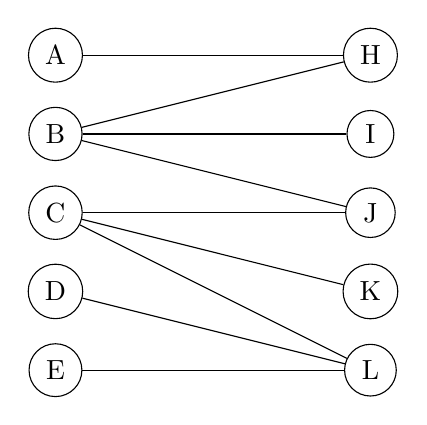
\begin{tikzpicture}
    \node[shape=circle,draw=black] (A) at (0,0) {A};
    \node[shape=circle,draw=black] (B) at (0,-1) {B};
    \node[shape=circle,draw=black] (C) at (0,-2) {C};
    \node[shape=circle,draw=black] (D) at (0,-3) {D};
    \node[shape=circle,draw=black] (E) at (0,-4) {E};
    \node[shape=circle,draw=black] (H) at (4,0) {H};
    \node[shape=circle,draw=black] (I) at (4,-1) {I};
    \node[shape=circle,draw=black] (J) at (4,-2) {J};
    \node[shape=circle,draw=black] (K) at (4,-3) {K};
    \node[shape=circle,draw=black] (L) at (4,-4) {L};
    \draw (A) -- (H);
    \draw (B) -- (H);
    \draw (B) -- (I);
    \draw (B) -- (J);
    \draw (C) -- (J);
    \draw (C) -- (K);
    \draw (C) -- (L);
    \draw (D) -- (L);
    \draw (E) -- (L);
\end{tikzpicture}
\end{center}
\noindent
\begin{multicols}{2}
example of maximum bipartite matching:\\
\begin{center}
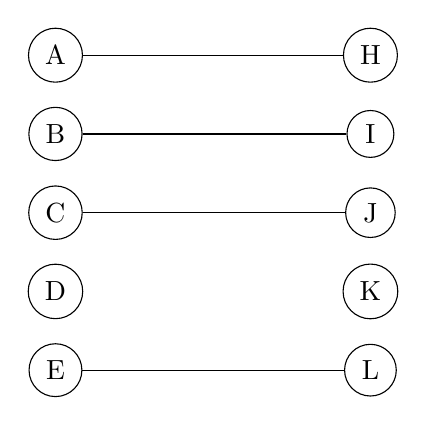
\begin{tikzpicture}
    \node[shape=circle,draw=black] (A) at (0,0) {A};
    \node[shape=circle,draw=black] (B) at (0,-1) {B};
    \node[shape=circle,draw=black] (C) at (0,-2) {C};
    \node[shape=circle,draw=black] (D) at (0,-3) {D};
    \node[shape=circle,draw=black] (E) at (0,-4) {E};
    \node[shape=circle,draw=black] (H) at (4,0) {H};
    \node[shape=circle,draw=black] (I) at (4,-1) {I};
    \node[shape=circle,draw=black] (J) at (4,-2) {J};
    \node[shape=circle,draw=black] (K) at (4,-3) {K};
    \node[shape=circle,draw=black] (L) at (4,-4) {L};
    \draw (A) -- (H);
    \draw (B) -- (I);
    \draw (C) -- (J);
    \draw (E) -- (L);
\end{tikzpicture}
\end{center}
\columnbreak
exapmle of maximal bipartite matching:\\
\begin{center}
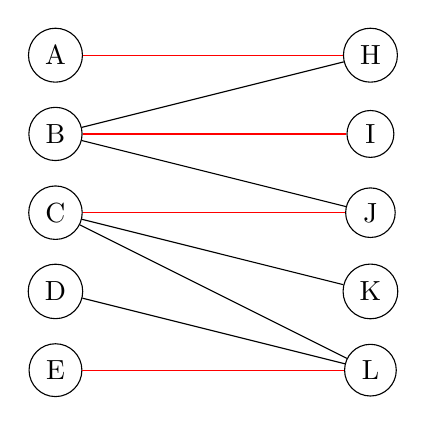
\begin{tikzpicture}
    \node[shape=circle,draw=black] (A) at (0,0) {A};
    \node[shape=circle,draw=black] (B) at (0,-1) {B};
    \node[shape=circle,draw=black] (C) at (0,-2) {C};
    \node[shape=circle,draw=black] (D) at (0,-3) {D};
    \node[shape=circle,draw=black] (E) at (0,-4) {E};
    \node[shape=circle,draw=black] (H) at (4,0) {H};
    \node[shape=circle,draw=black] (I) at (4,-1) {I};
    \node[shape=circle,draw=black] (J) at (4,-2) {J};
    \node[shape=circle,draw=black] (K) at (4,-3) {K};
    \node[shape=circle,draw=black] (L) at (4,-4) {L};
    \draw (A) -- (H);
    \draw (B) -- (H);
    \draw (B) -- (I);
    \draw (B) -- (J);
    \draw (C) -- (J);
    \draw (C) -- (K);
    \draw (C) -- (L);
    \draw (D) -- (L);
    \draw (E) -- (L);
    \draw[red] (A) -- (H);
    \draw[red] (B) -- (I);
    \draw[red] (C) -- (J);
    \draw[red] (E) -- (L);
\end{tikzpicture}
\end{center}
\end{multicols}
\noindent
From matchings to flows:\\
\begin{center}
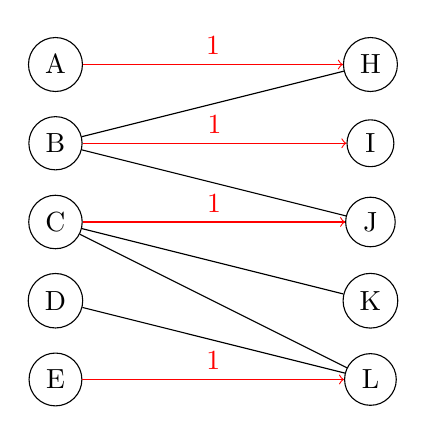
\begin{tikzpicture}
    \node[shape=circle,draw=black] (A) at (0,0) {A};
    \node[shape=circle,draw=black] (B) at (0,-1) {B};
    \node[shape=circle,draw=black] (C) at (0,-2) {C};
    \node[shape=circle,draw=black] (D) at (0,-3) {D};
    \node[shape=circle,draw=black] (E) at (0,-4) {E};
    \node[shape=circle,draw=black] (H) at (4,0) {H};
    \node[shape=circle,draw=black] (I) at (4,-1) {I};
    \node[shape=circle,draw=black] (J) at (4,-2) {J};
    \node[shape=circle,draw=black] (K) at (4,-3) {K};
    \node[shape=circle,draw=black] (L) at (4,-4) {L};
    \draw (A) -- (H);
    \draw (B) -- (H);
    \draw (B) -- (I);
    \draw (B) -- (J);
    \draw (C) -- (J);
    \draw (C) -- (K);
    \draw (C) -- (L);
    \draw (D) -- (L);
    \draw (E) -- (L);
    \draw[red] (A) -- (H);
    \draw[red] (B) -- (I);
    \draw[red] (C) -- (J);
    \draw[red] (E) -- (L);
    \draw[->,red] (A) -- (H) node[midway,above] {1};
    \draw[->,red] (B) -- (I) node[midway,above] {1};
    \draw[->,red] (C) -- (J) node[midway,above] {1};
    \draw[->,red] (E) -- (L) node[midway,above] {1};
\end{tikzpicture}
\end{center}
\noindent
\begin{center}
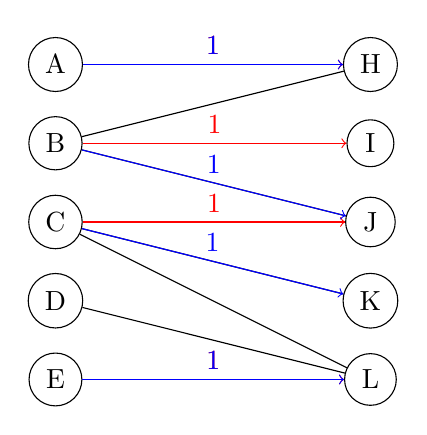
\begin{tikzpicture}
    \node[shape=circle,draw=black] (A) at (0,0) {A};
    \node[shape=circle,draw=black] (B) at (0,-1) {B};
    \node[shape=circle,draw=black] (C) at (0,-2) {C};
    \node[shape=circle,draw=black] (D) at (0,-3) {D};
    \node[shape=circle,draw=black] (E) at (0,-4) {E};
    \node[shape=circle,draw=black] (H) at (4,0) {H};
    \node[shape=circle,draw=black] (I) at (4,-1) {I};
    \node[shape=circle,draw=black] (J) at (4,-2) {J};
    \node[shape=circle,draw=black] (K) at (4,-3) {K};
    \node[shape=circle,draw=black] (L) at (4,-4) {L};
    \draw (A) -- (H);
    \draw (B) -- (H);
    \draw (B) -- (I);
    \draw (B) -- (J);
    \draw (C) -- (J);
    \draw (C) -- (K);
    \draw (C) -- (L);
    \draw (D) -- (L);
    \draw (E) -- (L);
    \draw[red] (A) -- (H);
    \draw[red] (B) -- (I);
    \draw[red] (C) -- (J);
    \draw[red] (E) -- (L);
    \draw[->,red] (A) -- (H) node[midway,above] {1};
    \draw[->,red] (B) -- (I) node[midway,above] {1};
    \draw[->,red] (C) -- (J) node[midway,above] {1};
    \draw[->,red] (E) -- (L) node[midway,above] {1};
    \draw[->,blue] (A) -- (H) node[midway,above] {1};
    \draw[->,blue] (B) -- (J) node[midway,above] {1};
    \draw[->,blue] (C) -- (K) node[midway,above] {1};
    \draw[->,blue] (E) -- (L) node[midway,above] {1};
\end{tikzpicture}
\end{center}
\noindent
\textbf{Maximum Flow and Maximum Matching}\\
The size of the maximum matching is equal to the value of the maximum flow.\\
The edges of $M$ are the edges that carry flow form $A$ to $B$ in the residual network.\\
Running time: $O(mn)$\\
\textbf{Baseball Elimination}
\begin{itemize}
    \item Given a set $S$ of teams
    \item For each team $x$ in $S$, the current number of wins $w_x$
    \item For teams $x$ and $y$ in $S$, they still have to play $g_{xy}$ games against each other
    \item Given a designated team $z$
    \item Can $z$ still win the turnament?
\end{itemize}
\textbf{From Baseball Elimination to flows}
\begin{itemize}
    \item For each pair of teams $x$ and $y$, create a vertex $v_{xy}$
    \item For each team $x$, create a vertex $v_x$
    \item For each pair of teams $x$ and $y$, create an edge $(s, v_{xy})$ with capacity $g_{xy}$
    \item For each team $x$, create an edge $(v_x, t)$ with capacity $w_z + g_{xz} - w_x$
    \item For each pair of teams $x$ and $y$, create an edge $(v_{xy}, v_x)$ with infinite capacity
    \item For each pair of teams $x$ and $y$, create an edge $(v_{xy}, v_y)$ with infinite capacity
\end{itemize}
\noindent
\textbf{Open pit mining}
\begin{itemize}
    \item Given a set $S$ of blocks
    \item For each block $x$ in $S$, the value $v_x$ of the ore in the block
    \item For each block $x$ in $S$, the cost $c_x$ of mining the block
    \item For each block $x$ in $S$, the set $N_x$ of blocks that are neighbors of $x$
    \item Given a designated block $z$
    \item What is the maximum value of ore that can be mined?
\end{itemize}
\textbf{From open pit mining to flows}
\begin{itemize}
    \item For each block $x$ in $S$, create a vertex $v_x$
    \item For each block $x$ in $S$, create an edge $(s, v_x)$ with capacity $v_x$
    \item For each block $x$ in $S$, create an edge $(v_x, t)$ with capacity $c_x$
    \item For each block $x$ in $S$, create an edge $(v_x, v_y)$ with infinite capacity for each block $y$ in $N_x$
\end{itemize}

\chapter{NP-Completeness}
\section{NP-Completeness}
\textbf{Polynomial time reduction}
\begin{itemize}
    \item Given a problem $A$ to solve
    \item Reduce solving $A$ to solving $B$
    \item Assume there is an algorithm $ALG^B$ that solves $B$ at cost $O(1)$
    \item Construct an algorithm $ALG^A$ that solves $A$, which uses $ALG^B$ as a subroutine
    \item If $ALG^A$ runs in polynomial time, then this is a polynomial time reduction
\end{itemize}
\textbf{How to work with reductions}\\
Positive: Assume that I want to solve problem $A$ and I know how to solve problem $B$.\\
\indent I can try come up with a polynomial time reduction $A \leq^p B$, which will give me a polynomial time algorithm for $A$.\\
Contrapositive: Assume that there is a problem $A$ for which it is unlikely that there is a polynomial time algorithm that solves $A$.\\
\indent If I come up with a polynomial time reduction $A \leq^p B$, it is also unlikely that there is a polynomial time algorithm that solves $B$.\\
\indent $B$ is "at least as hard to solve as" $A$, because if I could solve $B$, I could also solve $A$.\\ 
\textbf{Types of reductions}
\begin{itemize}
    \item Turing reduction: $A \leq_T B$
    \begin{itemize}
        \item A reduction which solves $A$ using (potentially many) calls to an oracle for $B$
        \item As known as Cook reduction
    \end{itemize}
    \item Many-one reduction: $A \leq_m B$
    \begin{itemize}
        \item A reduction which converts instances of $A$ to instances of $B$
        \item Also known as Karp reduction
    \end{itemize}
\end{itemize}
\textbf{Problem classification}\\
Problems in $P$:\\
\indent Searching, sorting, minimum spanning tree, graph traversal, maximum flow, minimum cut, weighted interval scheduling, etc.\\
Problems in $NP$:\\
\indent subset sum, knapSack, weighted interval scheduling, Searching, sorting, minimum spanning tree, graph traversal, maximum flow, minimum cut, etc.\\
\textbf{NP-hardness}\\
A problem $B$ is NP-hard if for every problem $A$ in $NP$, $A \leq^p B$.\\
\indent If every problem in $NP$ is polynomial time reducible to $B$, then this captures the fact that $B$ is at least as hard as any problem in $NP$.\\
\textbf{3 SAT}
\begin{itemize}
    \item A CNF formula with $m$ clauses and $k$ literals.
    \begin{equation*}
        \varphi = (x_1 \lor \lnot x_5 \lor x_3) \land ( x_2 \lor x_6 \lor \lnot x_5) \land \dots \land (x_3 \lor x_8 \lor x_{12})
    \end{equation*}
    \item each clause has exactly three literals
    \item Truth assignment: A value in $\{0, 1\}$ for each variable $x_i$
    \item Satisfying assignment: A truth assignment which makes the formula evaluate to $1$
    \item Computational problem 3 SAT: Decide if the input formula $\varphi$ has a satisfying assignment.
\end{itemize}
\textbf{3 SAT is NP-complete}
\begin{itemize}
    \item 3 SAT is in $NP$
    \begin{itemize}
        \item Given a truth assignment, we can check in polynomial time if it is satisfying
    \end{itemize}
    \item 3 SAT is NP-hard
    \begin{itemize}
        \item Given a CNF formula $\varphi$, we can construct a polynomial time reduction to 3 SAT
    \end{itemize}
\end{itemize}
\textbf{Proving NP-completeness}
\indent Suppose that you are given a problem $A$ and you want to prove that $A$ is NP-complete.\\
\indent First, prove that $A$ is in $NP$.\\
\indent \indent Usually by observing that a solution is efficiently verifiable.\\
\indent Then prove that $A$ is NP-hard.\\
\indent \indent construct a polynomial time reduction from a known NP-complete problem $P$.\\

\section{NP-completeness of the vertex cover problem}
\textbf{Vertex cover}
Definition: A vertex cover $C$ of a graph $G = (V, E)$ is a subset of vertices $C \subseteq V$ such that for every edge $e$ in $E$, at least one of the endpoints of $e$ is in $C$.\\
Definition: A minimum vertex cover is a vertex cover of smallest possible size.\\
Input: A graph $G = (V, E)$\\
Output: A minimum vertex cover\\
\textbf{Example}
\begin{center}
    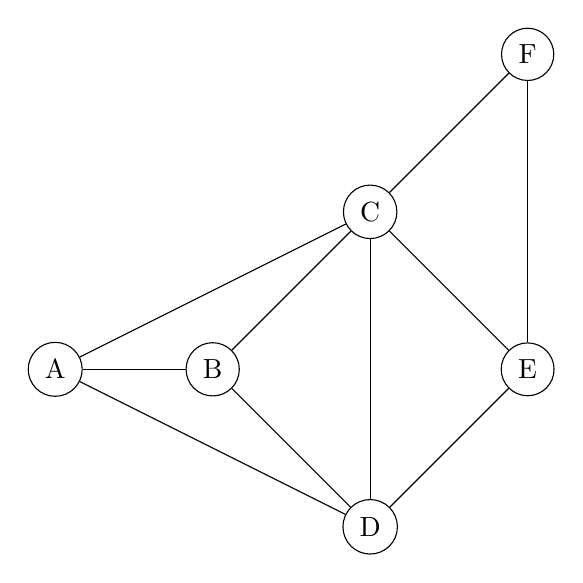
\begin{tikzpicture}
        \node[shape=circle,draw=black] (A) at (0, 0) {A};
        \node[shape=circle,draw=black] (B) at (2, 0) {B};
        \node[shape=circle,draw=black] (C) at (4, 2) {C};
        \node[shape=circle,draw=black] (D) at (4, -2) {D};
        \node[shape=circle,draw=black] (E) at (6, 0) {E};
        \node[shape=circle,draw=black] (F) at (6, 4) {F};
        \draw (A) -- (B);
        \draw (A) -- (C);
        \draw (A) -- (D);
        \draw (B) -- (C);
        \draw (B) -- (D);
        \draw (C) -- (D);
        \draw (C) -- (E);
        \draw (C) -- (F);
        \draw (D) -- (E);
        \draw (E) -- (F);
    \end{tikzpicture}\\
    the vertex cover $\{A, C, E\}$ is not a minimum vertex cover\\
    the minimum vertex cover is $\{A, E\}$.
\end{center}
\textbf{Vertex cover is NP-hard}: construct a polynomial time reduction from 3 SAT to vertex cover.\\
\indent Let $\varphi$ be a 3 CNF formula with $m$ clauses and $d$ variables.\\
\indent Construct in polynomial time an instance $<G, k>$ of vertex cover, with $k = d + 2m$.\\
\indent \indent if $\varphi$ is satisfiable, then $G$ has a vertex cover of size at most $k$\\
\indent \indent \indent Let $(y_1, y_2, \dots, y_d)$ in $\{0, 1\}^d$ be a satisfying assignment for $\varphi$\\
\indent \indent \indent For the nodes on the top: If $y_i = 1$. Include node $x_i$ in the vertex cover $C$, otherwise include node $\lnot x_i$ in $C$.\\
\indent \indent \indent For the nodes on the bottom: in each triangle, choose a node $x_i$ that has been picked on the top and do not include it in the vertex cover. Include the other two nodes.\\
\indent \indent if $\varphi$ is not satisfiable, then $G$ has no vertex cover of size at most $k$\\
\indent \indent \indent Let $C$ be a vertex cover of size $k = d + 2m$ in $G$.\\
\indent \indent \indent Since it is a vertex cover, it must include at least two out of three nodes in each "clause gadget" at the bottom.\\
\indent \indent \indent this means that at most $d$ nodes can be picked on the top.\\
\indent \indent \indent To satisfy the edges at the top, in each "variable gadget", at least one node must be picked.\\

\section{Further reductions in NP}
\textbf{Form optimization to decision}\\
Given an optimization problem $P$, introcude a threshold $k$.\\
The decision version $P_d$ becomes: Given an instance of $P$ and the threshold $k$ as input, is there a solution to $P$ with value at most $k$?\\
\indent If $P$ solved in polynomial time, then $P_d$ is also solved in polynomial time.\\
\indent If $P_d$ solved in polynomial time, then $P$ is also solved in polynomial time.\\
\noindent
\textbf{NP-complete problems}\\
Independent Set in graph $G$: A set of nodes in the graph, such that there is no edge between any two nodes in the set.\\
Maximum Independent Set: Given a graph $G$, find an independent set of maximum size.\\
Maximum Independent Set(desision version): Given a graph $G$ and a threshold $k$, is there an independent set of size at least $k$?\\
Set Packing: Given a set $U$ and a collection of subsets $S_1, S_2, \dots, S_m$ of $U$ and a number $k$, does there exist a collection of at least $k$ of these subsets that no two of them intersect?\\
Set Cover: Given a set $U$ and a collection of subsets $S_1, S_2, \dots, S_m$ of $U$ and a number $k$, does there exist a collection of at most $k$ of these sets whose union is $U$?\\
3-Dimensional Matching: Given three disjoint sets $X, Y, Z$ each of size $n$, and a collection of triples $T \subseteq X \times Y \times Z$, does there exist a set of $n$ triples in $T$, so that each element of $X \cup Y \cup Z$ appears in exactly one of these triples?\\
K-Colouring of a graph $G$: A function $f: V \rightarrow \{1, 2, \dots, k\}$ so that for every edge $(u, v)$ in $E$, $f(u) \neq f(v)$.\\
3-Colouring: Given a graph $G$, can we colour the nodes of $G$ using 3 colours so that no two adjacent nodes have the same colour?\\
Hamiltionian cycle in a directed graph $G$: A cycle in a directed graph that visits every node exactly once.\\
Hamiltionian path in a directed graph $G$: A path in a directed graph that contains every node exactly once.\\
Hamiltionian Cycle: Given a directed graph $G$, does $G$ contain a Hamiltionian cycle?\\
Hamiltionian Path: Given a directed graph $G$, does $G$ contain a Hamiltionian path?\\
Traveling Salesman: Given a complete graph $G$ with edge weights, and a threshold $k$, is there a tour of $G$ with total weight at most $k$?\\
\noindent
A texonomy of NP-complete problems\\
\indent Packing problems: Independent Set, Set Packing\\
\indent Covering problems: Vertex Cover, Set Cover\\
\indent Partitioning problems: 3-Dimensional Matching, Graph Colouring\\
\indent Sqequcen problems: Hamiltionian Cycle, Hamiltionian Path, Traveling Salesman\\
\indent Numerical problems: Subset Sum, Knapsack\\
\indent Constraint satisfaction problems: 3 SAT\\

\chapter{Liner Programming}
\textbf{Problem}: A company makes two products, $X$ and $Y$. Each product requires time on two machines, $A and B$.
\begin{itemize}
    \item Each unit of $X$ requires 50 minutes on machine $A$ and 30 minutes on machine $B$.
    \item Each unit of $Y$ requires 24 minutes on machine $A$ and 33 minutes on machine $B$.
    \item At the start of the week, there are 30 units of $X$ and 90 units of $Y$ in stock.
    \item The available processing time on machine $A$ is 40 hours, and on machine $B$ is 35 hours.
    \item The demand for $X$ in this week is 75 units, and for $Y$ is 95 units.
\end{itemize}
\textbf{Goal}: Maximise the combine sum of units of $X$ and $Y$ in stock at the end of the week.
\begin{align*}
    maximise(x+30-75)+(y+90-95)=x+y-50
\end{align*}
Base in the Description, we can get the following equations:
\begin{align*}
    \text{maximize  } \:& x+y-50\\
    \text{subject to  } \:& 50x+24y \leq 2400\\
    & 30x+33y \leq 2100\\
    & x \leq 45\\
    & y \leq 5\\
\end{align*}
\textbf{Solving the linear program}\\
\begin{center}
    \begin{tikzpicture}[scale=0.05]
        % draw the axis
        \draw[->] (0,0) -- (100,0) node[right] {$x$};
        \draw[->] (0,0) -- (0,100) node[above] {$y$};
        % draw the equations
        \draw[domain=0:65,smooth,variable=\x,black] plot ({\x},{100-(50/24)*\x});
        \draw[domain=0:75,smooth,variable=\x,black] plot ({\x},{(2100/33)-(30/33)*\x});
        \draw[domain=0:100,smooth,variable=\x,black] plot ({\x},{5});
        \draw[domain=0:100,smooth,variable=\x,black] plot ({45},{\x}); 
    \end{tikzpicture}
\end{center}

\section{Linear Programming}
\begin{align*}
    \text{maximize  } \:& \sum_{j=1}^n c_jx_j\\
    \text{subject to  } \:& \sum_{j=1}^n a_{ij}x_j \leq b_i \text{ for } i=1, 2, \dots, m\\
    & x_j \geq 0 \text{ for } j=1, 2, \dots, n
\end{align*}
\textbf{matrix form}
\begin{align*}
    \text{maximize  } \:& \mathbf{c}^T\mathbf{x}\\
    \text{subject to  } \:& \mathbf{Ax} \leq \mathbf{b}\\
    & \mathbf{x} \geq \mathbf{0}
\end{align*}
\noindent
\textbf{Solving the linear program}
\begin{itemize}
    \item To find the optimal solution, it suffices to examine the conrners of the feasible region.
    \item These are the intersection points of the lines defined by the constraints.
    \item This is the Simplex method.
    \item Otehr algorithm for solving LPs: Ellipsoid method, Interior point method.
\end{itemize}
\textbf{Integer Linear Programming}\\
\begin{align*}
    \text{maximize  } \:& \sum_{j=1}^n c_jx_j\\
    \text{subject to  } \:& \sum_{j=1}^n a_{ij}x_j \leq b_i \text{ for } i=1, 2, \dots, m\\
    & x_j \geq 0 \text{ for } j=1, 2, \dots, n\\
    & x_j \in \mathbb{Z} \text{ for } j=1, 2, \dots, n
\end{align*}
\textbf{Solving the integer linear program}\\
The corners are not necessarily integer solutions. it does not suffices to look at the corners.\\
WE can exhaustively search all possible integer solutions.\\
Generally, this is NP-hard.\\

\begin{enumerate}
    \item Linear Programming can be solved in polynomial time.
    \item Integer Linear Programming Generally cannot be solved in polynomial time.(unless P=NP)
\end{enumerate}

\section{Duality}
\begin{itemize}
    \item Suppose that we have a linear program, which we call the primal.
    \item We will construct another linear program, which we call the dual.
    \item The variables of the primal become the constraints of the dual, and vice versa.
    \item Maximisation becomes minimisation.
    \item The two linear programs will have a very important connection.
\end{itemize}
\textbf{Primal}
\begin{align*}
    \text{maximize  } \:& \sum_{j=1}^n c_jx_j\\
    \text{subject to  } \:& \sum_{j=1}^n a_{ij}x_j \leq b_i \text{ for } i=1, 2, \dots, m\\
    & x_j \geq 0 \text{ for } j=1, 2, \dots, n
\end{align*}
\textbf{Dual}
\begin{align*}
    \text{minimize  } \:& \sum_{i=1}^m b_iy_i\\
    \text{subject to  } \:& \sum_{i=1}^m a_{ij}y_i \geq c_j \text{ for } j=1, 2, \dots, n\\
    & y_i \geq 0 \text{ for } i=1, 2, \dots, m
\end{align*}
\noindent
\textbf{Weak Duality}\\
Let $\mathbf{x}$ be any feasible solution to the primal, and let $\mathbf{y}$ be any feasible solution to the dual. Then
\begin{align*}
    value(\mathbf{x}) \leq value(\mathbf{y})
\end{align*}
\textbf{Strong Duality}\\
Let $\mathbf{x}$ be any feasible solution to the primal, and let $\mathbf{y}$ be any feasible solution to the dual. if 
\begin{align*}
    value(\mathbf{x}) = value(\mathbf{y})
\end{align*}
then $\mathbf{x}$ and $\mathbf{y}$ are optimal solutions to the primal and dual respectively.\\
\noindent
\textbf{LP-relaxation}\\
An LP-relaxation of an integer linear program is a linear program which is identical to the integer linear program, except all the integrality constraints have been removed, or replaced with non-negativity constraints.\\
Example of Minimum Cut as ILP and LP-relaxation\\
\begin{align*}
    \text{minimize  } \:& \sum_{(u,v) \in E} c_{uv}d_{uv}\\
    \text{subject to  } \:& d_{uv} - z_u + z_v \geq 0 \text{ for each } (u,v) \in E,u \neq s, v \neq t\\
    & d_{su} +z_u \geq 0 \text{ for each} (s,u) \in E\\
    & d_{ut} - z_u \geq 0 \text{ for each} (u,t) \in E\\
    & d_{uv} \geq 0 \text{ for each } (u,v) \in E\\
    & z_u \in \{0,1\} \text{ for each } u \in V-\{s,t\}\\
\end{align*}




\chapter{Approximation Algorithms}
\section{Approximation Algorithms}
\textbf{Why Approximation Algorithms?}
\begin{itemize}
    \item For some problems, there is no known polynomial time algorithm.
    \item We can design an approximation algorithm
    \begin{itemize}
        \item It runs in polynomial time
        \item Compute a solution that is guaranteed to be close to the optimal solution
    \end{itemize}
\end{itemize}
\textbf{Methods of approximation algorithms}
\begin{itemize}
    \item Greedy algorithms
    \item Linear programming and rounding
    \item Pricing method
    \item Dynamic programming on round inputs
\end{itemize}
\textbf{Application: Load Balancing}
\begin{itemize}
    \item We have a set of $m$ identical machines $M_1, M_2, \dots, M_m$.
    \item We have a set of $n$ jobs, with job $j$ having processing time $t_j$.
    \item We want to assign each job to some machine.
    \item Let $A(i)$ be the set of jobs assigned to machine $i$
    \item The load of machine $i$ is $T(i) = \sum_{j \in A(i)} t_j$
    \item The goal is to minimize the makespan,i.e, $T=\max_i T(i)$
\end{itemize}
The load balancing problem is NP-hard.\\
\textbf{Greedy Algorithm}
\begin{itemize}
    \item Pick any job
    \item Assign it to the machine with the smallest load so fraction
    \item Remove it from the pile of jobs
\end{itemize}
\textbf{Arguing about the optimal}
\begin{itemize}
    \item we want to prove that $T$ os not far from $T^*$
    \item We will show that $T$ is not far from something which is samller than $T^*$
    \item Then it is certainly not far from $T^*$
    \item Fundamental idea: Bounding the optimal from below (for minimisation problems) and from above (for maximisation problems).
\end{itemize}
Consider the total processing time of all jobs.(the sum of all $t_j$).\\
\indent one of the $m$ machines must be allocated at least $\frac{1}{m}$ of the total work.\\
\indent we have that $T^* \geq \frac{1}{m} \sum_{j=1}^n t_j$\\
Every job must be scheduled on some machine.\\
\indent the makespan is certainly at least the largest processing time $t_j$ of any job.\\
\indent we have that $T^* \geq \max_j t_j$\\

\noindent
\textbf{The Proof}\\
\indent Consider the final job $j$ assigned to machine $M_i$ by the greedy algorithm. Consider the time when this assignment is made.\\
\indent This was the smallest load among all machines.\\
\indent Every other machine had load at least $T_i-t_j$ at this time.\\
\indent Summing up over all machines, we get 
\begin{align*}
    \sum_k T_k \geq m(T_i-t_j) \Rightarrow T_i-t_j \leq \frac{1}{m} \sum_k T_k
\end{align*}
\indent So we got the first lower bound.\\
\begin{align*}
    T^* \geq T_i - t_j (\text{first lower bound})
\end{align*}
Consider a job $j$ assigned to machine $M_i$ by the greedy algorithm. Consider the time when this assignment took place.\\
\indent The load of machine $j$ was $T_i-t_j$.\\
\indent This was before we added the job.\\
\indent After we add the job, the load is $T_i-t_j+t_j$.\\
\indent Obviously, $t_j \leq \max_k t_k \leq T^*$.\\
\indent Since $T^*$ is the optimal makespan, it must be at least as large as the load of the machine with the largest load.\\
\indent So we got the second lower bound.\\
\begin{align*}
    t_j \leq T^* (\text{second lower bound})
\end{align*}
\indent Combining the two lower bounds, we get
\begin{align*}
    T_i \leq 2T^* (\text{since j was the final job})
\end{align*}

\textbf{Approximation Ratio}\\
Consider a minimization problem $P$ and an objective $obj$.\\
\indent Here: Load Balancing on identical machines, and makespan.
\begin{itemize}
    \item Consider an approximation algorithm $A$.
    \item Consider an input $x$ to $P$.
    \item Let $obj(A(x))$ be the value of the objective function on the output of $A$.
\end{itemize}
The approximation ratio of $A$ is defined as
\begin{align*}
    \max_{x \in \text{all inputs}} \frac{obj(A(x))}{obj(x)}
\end{align*}
\begin{itemize}
    \item In order to prove an upper bound on the approximation ratio, we have to somehow argue about all inputs.
    \item In order to prove a lower bound on the approximation ratio, we have to argue about a specific input.
\end{itemize}
For maximum problems, we define the approximation ratio as
\begin{align*}
    \max_x \frac{obj(x)}{obj(A(x))}
\end{align*}
For minimization problems, we define the approximation ratio as
\begin{align*}
    \max_x \frac{obj(A(x))}{obj(x)}
\end{align*}
Convention, to have approximation ratio always $\geq 1$.\\
A better greedy algorithm for load balancing\\
\begin{itemize}
    \item Sort the jobs in decreasing order of processing times.
    \item Pick a job and according to this order.
    \item Assign it to the machine with the smallest load so far.
    \item Remove it from the pile of jobs.
\end{itemize}
\begin{algorithm}[H]
\caption{Greedy Algorithm for Load Balancing}
\begin{algorithmic}[1]
\State Sort the jobs in decreasing order of processing times.
\State $T \gets 0$
\For{$j=1$ to $n$}
\State Assign job $j$ to the machine with the smallest load so far.
\State $T \gets \max(T,T(i))$
\EndFor
\State \Return $T$
\end{algorithmic}
\end{algorithm}
\noindent
Consider a job $j$ that was assigned to machine $M_i$ by the greedy algorithm. Consider the time when this assignment took place.\\
\indent The load of machine $j$ was $T_i-t_j$.\\
\indent This was before we added the job.\\
\indent After we add the final job, the load is $T_i-t_j+t_j$.\\
\indent we established that $t_j \leq t_{m+1} \leq \frac{1}{2} T^*$.\\
\indent Now we have the third lower bound.\\
\begin{align*}
    t_j \leq \frac{1}{2} T^* (\text{third lower bound})
\end{align*}
\indent Combining the three lower bounds, we get
\begin{align*}
    T_i \leq \frac{3}{2} T^* \\
    \Rightarrow T \leq \frac{3}{2} T^*
\end{align*}
The approximation ratio of the greedy algorithm actually is $\frac{4}{3}$ with a better analysis.\\
For the loading balancing problem on identical machines, there is a Polynomial time approximation scheme (PTAS).\\
\indent An algorithm which, given an input and a parameter $\epsilon$, runs in polynomial time and produces an outcome which is $1+\epsilon$ far from the optimal.\\
\noindent
\textbf{Inapproximability}\\
A PTAS (or an FPTAS, more on that later) is the best approximation we can hope for, for an NP-hard problem.\\
Often it is not possible to get that close.\\
\indent Inapproximability $\alpha$ of a problem $P$:\\
\indent \indent There is no polynomial time algorithm that achieves an approximation ratio better than $\alpha$.\\

\section{The traveling salesman problem}
Problem definition:\\
\indent $n$ cities, $c_{ij}$ is the cost of traveling from city $i$ to city $j$.\\
\indent $c_{ij} = c_{ji} \geq 0,c_{ii} = 0$\\
Feasible solution: A tour that visits every city exactly once and returns to the starting city.\\
Optimal solution: A feasible tour with minimum total cost.\\
\textbf{Graph interpretation}\\
Complete graph on $n$ vertices.\\
\indent $c_{ij}$ is the weight of the edge $(i,j)$.\\
Tour: Hamiltonian cycle in the graph.\\
Goal: A Hamiltonian cycle with minimum total weight.\\
Mtetric TSP problem: The cost satisfy the triangle inequality.\\
\begin{equation*}
    c_{ik} \leq c_{ij} + c_{jk}
\end{equation*}
\textbf{The Nears Neighbor Algorithm}
\begin{itemize}
    \item Start with a greedy step
    \item Start with an edge $(i,j)$ of minimum weight.
    \item Create a cycle$(i,j,i)$.
\end{itemize}
Generally, Assume that we have already visited a set of cities $S$. We find a city $i \in S$ and a city $j \notin S$ such that the cost of the edge $(i,j)$ is minimum possible. We include $j$ in $S$ and insert it between $i$ and the city that follows $i$ in the cycle.\\
Consider the tour $(u_1,u_2,\dots,u_n)$ and remove the final that brings us back to $u_1$. We will have a spanning tree. So the cost of the tour is at least the cost of the spanning tree.\\
\textbf{Lemma}: cost(optimal tour) $\geq$ cost(minimum spanning tree).\\
We can use Prim Algorithm to find the minimum spanning tree.\\
Let $F=\{(u_2,v_2),(u_3,v_3),\dots,(u_{n},v_{n})\}$ be the set of edges in the minimum spanning tree.\\
\begin{equation*}
    \text{Hence} OPT \geq \sum_l c_{u_l,v_l}
\end{equation*}
The cost of the algorithm is at most $2 \sum_l c_{u_l,v_l}$.\\
The cost of the tour between first two nodes is $2c_{u_1,v_1}$.\\
When inserting the city $j$, the cost increases by $c_{i,j}+c_{j,k}-c_{i,k} \leq c_{i,j}+c_{i,k}-c_{i,k} = 2c_{i,j}$.\\
\textbf{A different perspective}
\begin{itemize}
    \item Start by finding a minimum spanning tree.
    \item Duplicate each edge of the tree.
    \item Do a traversal following the edges of the tree.
    \item Turn this into a tour by shortcutting.
\end{itemize}

\indent \textbf{Eulerian Graph}\\
\indent There is a permutation of the edegs $(i_0,i_1),(i_1,i_2),\dots,(i_{k-1},i_k),(i_k,i_0)$. If this exists, we can make a traversal of the edegs, visiting each edge exactly once.\\
\indent Property: A graph is Eulerian if and only if it is connected and every vertex has even degree.\\
Some Facts:\\
\indent \textbf{Fact 1}: the sum of its degrees is even.\\
\indent \textbf{Fact 2}: The total number of even-degree nodes is an even number.\\
\indent \textbf{Fact 3}: The total number of odd-degree nodes is an even number.\\
\indent \textbf{Fact 4}: The number of odd-degree nodes is even.\\
Constructing an Eulerian graph:\\
\indent Start from the minimum spanning tree $T$.\\
\indent Consider the set of odd-degree nodes $O$.\\
\indent Find a minimum weight perfect matching of $O$. (This can be done in polynomial time.)\\
\indent Add the edges of the matching to $T$.\\
\indent The resulting graph is Eulerian.\\
Equivalently: The cost of the perfect matching is at most $OPT/2$.\\

\textbf{Bunding the cost of the perfect matching}\\
\indent Claim: There is partial tour containing the cities in $O$ that has cost at most $OPT$.\\
\indent \indent Consider the optimal tour.(on the whole graph)\\
\indent \indent Consider a part $(i,u_1,u_2,\dots,u_l,j)$ of the tour where the cities $u_1,u_2,\dots,u_l$ are in $O$.\\
\indent \indent "Shortcut" from $i$ to $j$ directly, without an increase in cost.\\
\indent The cheapest of those two has cost at most $OPT/2$.\\
\textbf{The approximation landscape of TSP}\\
\indent The $\frac{3}{2}$-approximation algorithm is due to Christofides (1976).\\
\indent Inapproximability: 1.0045.\\

\section{Primal-Dual Method}
Design a polynomial time apporximation algorithm for the weighted vertex cover problem.\\
\textbf{The Pricing Method}\\
\indent Consider a vertex cover $S$.\\
\indent Every vertex $i$ has a cost, which is equal to $w_i$.\\
\indent If $i \in S$, then the edges that "use it" have to pay for the cost.\\
\indent Each edge $e$ in the graph pays a price $p_e$.\\
Given a vertex cover $i$, we never ask the edges to pay more than the cost of $i$.\\
\begin{equation*}
    \sum_{e \in E} p_e \leq w_i
\end{equation*}
\textbf{Lemma}: Let $S$ be any vertex cover and let $p_e$ be any non-negative fair prices. Then ,it holds that:\\
\begin{equation*}
    \sum_{e \in E} p_e \leq w(S)
\end{equation*}
\textbf{Proof of Lemma}:\\
\begin{enumerate}
    \item By fairness, we have that: $\sum_{e=(i,j)} p_e \leq w_i$
    \item Adding up over all nodes, we have 
    \begin{equation*}
        \sum_{i \in S} \sum_{e=(i,j)} p_e \leq \sum_{i \in S} w_i = w(S)
    \end{equation*}
    \item Since $S$ is a vertex cover, each edge contributes at least one term $p_e$ to expression.
    \item From this, we get that
    \begin{equation*}
        \sum_{e \in E} p_e \leq \sum_{i \in S} \sum_{e=(i,j)} p_e
    \end{equation*}
\end{enumerate}
Terminology: We will say that a node $i$ is "tight" if $\sum_{e=(i,j)} p_e = w_i$.\\
\begin{algorithm}[H]
\caption{Vertex-Cover-Approximation(G,w)}
\begin{algorithmic}[1]
\State $p_e \gets 0$ for all $e \in E$
\While{there is an edge $e=(i,j)$ such that neither $i$ nor $j$ is tight}
    \State $p_e \gets \frac{w_i+w_j}{2}$
\EndWhile
\State $S \gets \{i: i \text{ is tight}\}$
\State \Return $S$
\end{algorithmic}
\end{algorithm}
\noindent
\textbf{second lemma}: The set $S$ and the prices $p$ returned by the Vertex-Cover-Approximation algorithm satisfy: 
\begin{equation*}
    w(S) \leq 2 \sum_{e \in E} p_e
\end{equation*}
\textbf{Proof of second lemma}:\\
\begin{enumerate}
    \item Consider a node $i$ in $S$.
    \begin{itemize}
        \item This means that $i$ is tight.
        \item This means that $\sum_{e=(i,j)} p_e = w_i$.
    \end{itemize}
    \item Summing up over all nodes in $S$, we get that
    \begin{equation*}
        w(S)=\sum_{i \in S} w_i = \sum_{i \in S} \sum_{e=(i,j)} p_e
    \end{equation*}
    \item An edge $e=(i,j)$ can be included in the sum at most twice.
    \item From this, we get that
    \begin{equation*}
        w(S)=\sum_{i \in S} \sum_{e=(i,j)} p_e \leq 2 \sum_{e \in E} p_e
    \end{equation*}
\end{enumerate}
\textbf{Correctness}:
\begin{enumerate}
    \item First,$S$ is a vertex cover.
    \item Suppose that it is not.
    \item Then there is an edge $e=(i,j)$ that is not covered by $S$.
    \item This means that neither $i$ nor $j$ is tight.
    \item The algorithm did not terminate, because of "while there is an edge $e=(i,j)$ such that neither $i$ nor $j$ is tight".
\end{enumerate}
\textbf{Approximation Ratio}:
\begin{itemize}
    \item Let $S^*$ be the mimimum weight vertex cover.
    \item Recall that $S$ is the vertex cover returned by the algorithm.
    \item we have:
    \begin{equation*}
        \sum_{e \in E} p_e \leq w(S^*) \text{                   and         }
        w(S) \leq 2 \sum_{e \in E} p_e
    \end{equation*}
    \item Combining the two, we get that $w(S) \leq 2w(S^*)$.
\end{itemize}
\textbf{Vertex Cover as an ILP}:\\
\begin{equation*}
    \begin{aligned}
    \text{minimize} \quad & \sum_{i \in V} w_i x_i\\
    \text{subject to} \quad & x_i + x_j \geq 1 \quad \forall (i,j) \in E\\
    & x_i \in \{0,1\} \quad \forall i \in V\\
    &x_i \geq 0 \quad \forall i \in V
    \end{aligned}
\end{equation*}
\textbf{Vertex Cover LP-relaxation}:\\
\begin{equation*}
    \begin{aligned}
    \text{minimize} \quad & \sum_{i \in V} w_i x_i\\
    \text{subject to} \quad & x_i + x_j \geq 1 \quad \forall (i,j) \in E\\
    & 0 \leq x_i \quad \forall i \in V
    \end{aligned}
\end{equation*}
\textbf{The Dual}
\begin{equation*}
    \begin{aligned}
    \text{maximize} \quad & \sum_{(i,j) \in E} y_{ij}\\
    \text{subject to} \quad & \sum_{(i,j) \in E} y_{ij} \leq w_i \quad \forall i \in V\\
    & y_{ij} \geq 0 \quad \forall (i,j) \in E
    \end{aligned}\\
    \begin{aligned}
    \text{maximize} \quad & \sum_{e \in E} p_e\\
    \text{subject to} \quad & \sum_{e=(i,j)} p_e \leq w_i \quad \forall i \in V\\
    & p_e \geq 0 \quad \forall e \in E
    \end{aligned}
\end{equation*}
\textbf{Primal-dual method}:\\
\begin{itemize}
    \item We start with an infeasible integral solution $x$ to the primal and a feasible fractional solution $y$ to the dual.
    \item We increase the value of some $y_j$ until some constraint becomes tight.
    \begin{itemize}
        \item We obtain a better feasible fractional solution $y$ to the dual.
        \item We increase the corresending variable $x_i$ of the primal to obtain a still feasible integral solution $x$ to the primal, which however violates fewer constraints.
    \end{itemize}
    \item We end up  with a feasible integral solution $x$ to the primal and a feasible fractional solution $y$ to the dual.
    \item We compare the two solutions.
\end{itemize}

\section{Rounding Linear Programs}
In last section, we designed an algorithm for the vertex cover problem, which used the following LP-relaxation:
\begin{equation*}
    \begin{aligned}
    \text{minimize} \quad & \sum_{i \in V} w_i x_i\\
    \text{subject to} \quad & x_i + x_j \geq 1 \quad \forall (i,j) \in E\\
    & 0 \leq x_i \quad \forall i \in V\\
    & x_i \in \{0,1\} \quad \forall i \in V
    \end{aligned}
\end{equation*}
\textbf{Solving the LP-relaxation}:\\
\begin{itemize}
    \item We can solve the LP-relaxation in polynomial time, to find an optimal solution.
    \item The optimal solution is a "fractional" vertex cover, where variables can take values between 0 and 1.
    \item Is the value of the "fractional" vertex cover, smaller or larger than the value of the mimimum weight vertex cover?
\end{itemize}
We do not know the optimal, so using a lower bound for the optimal.\\
Now we have a bound:
\begin{equation*}
    \text{optimal fractional VC weight} \leq \text{optimal VC weight} \leq \text{algorithm VC weight}
\end{equation*}
\textbf{Rounding the LP-relaxation}:\\
We round the fractional solution to an integral solution.
\begin{itemize}
    \item We pick a variable $x_i$ and round it to 0 or 1.
    \item If we set everything to 0, it is not a vertex cover.
    \item If we set everything to 1, we "pay" too much.
    \item We set variable $x_i$ to 1 if $x_i \geq 1/2$ and to 0 otherwise.
\end{itemize}
\textbf{Feasibility}:
Claim: The solution that we obtain is a vertex cover. This is, the round solution is a feasible solution to the ILP.
Easy Proof: Assume that it is not.
\begin{itemize}
    \item Then there is an edge $e=(i,j)$ such that both $x_i$ and $x_j$ are 0.
    \item This means that in the LP-relaxation, we have that $x_i < 1/2$ and $x_j < 1/2$.
    \item But then the constraint $x_i + x_j \geq 1$ would be violated, and this would not be a feasible solution to the LP-relaxation.
\end{itemize}
\textbf{Approximation Ratio}:
\begin{itemize}
    \item Claim: The vertex cover obtained from rounding has weight at most twice that of the minimum weight vertex cover.
    \item Intuition is easy: We included all the vertices for which the LP-relaxation "paid" at least 1/2, and we rounded them to 1, so we "paid" at most twice the optimal.
    \item One line proof: Let $x^*$ be the optimal solution to the LP-relaxation, then
    \begin{equation*}
        \sum_i w_i x_i^* \geq \sum_{i \in S} w_i x_i^* \geq \frac{1}{2} \sum_{i \in S} w_i = \frac{1}{2} w(S)
    \end{equation*}
\end{itemize}
The LP-relaxation and round algorithm for vertex cover has approximation ratio of 2. We already know that 2 was possible, from the Pricing method algorithm. In this case, the ILP-relaxation and round algorithm seems conceptually simpler. In other cases, rounding the solution will not be straightforward.\\
\textbf{Limitations of the techniques}\\
The LP-relaxation and round techniques cannot provide approximation ratios better than the integrality gap of the ILP-LP fomulation.\\
Caution: The integrality gap is a quantity has to do with the formulation of the ILP-LP, not the problem.
\begin{itemize}
    \item An integrality gap of $\alpha$ does not mean that it is not possible to design an algorithm with approximation ratio better than $\alpha$.
    \item actually, it does not even mean that LP-relaxation and round cannot give you an algorithm with approximation ratio better than $\alpha$.
    \item It means that with this formulation of the ILP-LP, $\alpha$ is the best approximation ratio that you can get.
\end{itemize}
\textbf{Inapproximability of VC}\\
\begin{itemize}
    \item We saw two different algorithms, both with an approximation ratio of 2.
    \item Could we hope to design a better algorithm?
    \item The answer to this question depends on our definition of "hope".
    \item \textbf{Known fact 1}: It is impossible to design an algorithm with approximation ratio better than 1.363, unless $P=NP$.
    \item \textbf{Known fact 2}: It is impossible to design an algorithm with approximation ratio better than 2, unless Unique Games is an NP hard problem.
    \item Both facts are quite involved to prove.
\end{itemize}
\textbf{Easier Inapproximability}\\
Definition: A problem $P$ is strongly NP-hard, when it has a polynomial time reduction from a strongly NP-hard problem.\\
For a strongly NP-hard problem
\begin{itemize}
    \item There is no Fully Polynomial Time Approximation Scheme (FPTAS).
    \item There is no pseudopolynomial time algorithm that solves it exactly.
    \subitem Equivalently, if it remains NP-complete even when all of its number parameters are bounded by a polynomial in the length of the input.
\end{itemize}
\textbf{VC on bipartite graphs}\\
Vertex Cover as an ILP:
\begin{equation*}
    \begin{aligned}
    \text{minimize} \quad & \sum_{i \in V} x_i\\
    \text{subject to} \quad & x_i + x_j \geq 1 \quad \forall (i,j) \in E\\
    & x_i \in \{0,1\} \quad \forall i \in V \\
    & x \geq 0 \quad \forall i \in V
    \end{aligned}
\end{equation*}
Vertex Cover as an LP-relaxation:
\begin{equation*}
    \begin{aligned}
    \text{minimize} \quad & \sum_{i \in V} x_i\\
    \text{subject to} \quad & x_i + x_j \geq 1 \quad \forall (i,j) \in E\\
    & x \geq 0 \quad \forall i \in V
    \end{aligned}
\end{equation*}
The dual of the LP-relaxation:
\begin{equation*}
    \begin{aligned}
    \text{maximize} \quad & \sum_{e \in E} y_e\\
    \text{subject to} \quad & y_e \leq 1 \quad \forall e \in E\\
    & y_e \geq 0 \quad \forall e \in E
    \end{aligned}
\end{equation*}
The ILP corresponding to the dual:
\begin{equation*}
    \begin{aligned}
    \text{maximize} \quad & \sum_{e \in E} y_e\\
    \text{subject to} \quad & \sum_{e=\{i,j\} \in E} y_e \leq 1 \quad \forall i \in V\\
    & y_e \in \{0,1\} \quad \forall e \in E
    \end{aligned}
\end{equation*}
\textbf{König's Theorem}\\
In a bipartite graph, the size of the maximum matching is equal to the size of the minimum vertex cover.
\begin{itemize}
    \item König's proof is constructive: It starts from a maximum matching, and constructs a minimum vertex cover, proving that it is minimum.
    \item Alternative proof based on total unimodularity.
\end{itemize}
So we have:
\begin{itemize}
    \item size of the maximum matching = size of the minimum vertex cover
    \item size of the minimum vertex cover = size of minimum fractional VC.
    \item size of the maximum fractional matching = size of the minimum fractional VC.
    \item size of maximum matching = size of minimum VC.
\end{itemize}
Solve for VC on bipartite graphs:
\begin{itemize}
    \item Pick a vertex $v$ in the graph.
    \item Remove it to get graph $G-\{v\}$.
    \item Property: If $v$ is in the minimum vertex cover, $G-\{v\}$ has a minimum vertex cover of size $k^*-1$.
    \item Check if the graph $G-\{v\}$ has a vertex cover of size at most $k^*-1$.
    \subitem Yes: Include $v$ in the vertex cover.
    \subitem No: Do not include $v$ in the vertex cover.
    \subitem Then move on to the next vertex.
\end{itemize}
\textbf{Summing up}\\
Vertex Cover is strongly NP-hard in general graphs.
\begin{itemize}
    \item In fact, hard to approximate better than 1.363.
    \item There exist 2-approximate polynomial time algorithms for the problem.
\end{itemize}
On bipartite graphs, the problem is solvable in polynomial time.


\section{Dynamic Programming on Rounded Inputs}
\textbf{The 0/1-Knapsack Problem}\\
Given a set of $n$ items $\{1,2,\dots,n\}$. Each item $i$ has a non-negative value $v_i$ and a non-negative weight $w_i$. We are given a bound $W$ on the total weight.\\
Goal: Select a subset of $S$ of items that $\sum_{i \in S} w_i \leq W$ and $\sum_{i \in S} v_i$ is maximized.\\
Dynamic Programming algorithm for 0/1-Knapsack:
\begin{algorithm}[H]
\caption{SubsetSum}
\begin{algorithmic}[1]
    \State $M=[0\dot n,0\dot W]$
    \State $M[0,0] \gets 0$
    \For{$i=1,\dots,n$}
        \For{$w=0,\dots,W$}
            \If{$w_i \leq w$}
                \State $M[i,w] \gets \max\{M[i-1,w], M[i-1,w-w_i]+v_i\}$
            \Else
                \State $M[i,w] \gets M[i-1,w]$
            \EndIf
        \EndFor
    \EndFor
    \State \Return $M[n,W]$
\end{algorithmic}
\end{algorithm}
\noindent
The dynamic programming algorithm for 0/1 knapsack solves knapsack optimally in time polynomial in $n$ and $W$.
\begin{algorithm}[H]
\caption{Knapsack($n,W$)}
\begin{algorithmic}[1]
    \State $M=[0\dot n,0\dot W]$
    \State $M[0,0] \gets 0$
    \For{$i=1,\dots,n$}
        \For{$w=0,\dots,W$}
            \If{$w_i \leq w$}
                \State $M[i,w] = M[i-1,w]$
            \Else
                \State $M[i,w] = \max\{M[i-1,w], M[i-1,w-w_i]+v_i\}$
            \EndIf
        \EndFor
    \EndFor
    \State \Return $M[n,W]$
\end{algorithmic}
\end{algorithm}
\noindent
Another pseudopolynomial time algorithm for 0/1-Knapsack
\begin{algorithm}[H]
\caption{Knapsack($n,W$)}
\begin{algorithmic}[1]
    \State $M=[0\dots n,0\dots V]$
    \State $M[i,0] \gets 0 \quad \forall i$
    \For {$i=1,\dots,n$}
        \State $S(i)=\sum_{j=1}^i v_j$
    \EndFor
    \For {$v=1,\dots,V$}
        \If {$v > S(n)$}
            \State $M[i,v]=w_i+M[i-1,v-v_i]$
        \Else
            \State $M[i,v]=\min\{w_i+M[i-1,v-v_i],M[i-1,v]\}$
        \EndIf
    \EndFor
    \State \Return $\max\{v \mid M[n,v] \leq W\}$
\end{algorithmic}
\end{algorithm}
\noindent
\textbf{Intuition}\\
We will create subproblems based on the values, not the weights.\\
Each subproblem will be defined by an index $i$ and target value $v$.\\
\indent $M[i,v]$ is the smallest knapSack weight $W$ such that it is possible to obtain a solution using a subset of items $\{1,\dots,i\}$ with total value at least $v$.\\
We have subproblems at most $(n^2v^*)$, where $v^*$ is the maximum value of any item.\\
\textbf{Information about knapSack}\\
A pseudo-polynomial time algorithm for solving the problem exactly(actually, a couple of those).\\
A polynomial time greedy approximation algorithm with approximation ratio $2$.\\
\textbf{Rounding the values}\\
Use a rounding parameter $b$.\\
For each item $i$, let $\tilde{v}_i = \lceil \frac{v_i}{b}*b \rceil$.\\
\indent It holds that for each item $i$, $v_i \leq \tilde{v}_i \leq v_i + b$.\\
\indent let $\hat{v}_i = \frac{\tilde{v}_i}{b}= \lceil \frac{v_i}{b} \rceil$.\\
We divide all the values by $b$ and round up.\\
\textbf{The algorithm}\\
knapsack-approx($\mathcal{E}$)
Set $b=\frac{\epsilon}{2n}\max_i v_i$\\
Run the DP algorithm for knapsack on values $\hat{v}_i$.\\
Return the set $S$ of items founds.\\
\textbf{Feasibility}\\
The set $S$ is a feasible solution to the knapsack, we didn't mess up the weights.\\
\textbf{Running time}\\
The DP algorithm runs in time $O(n^2v^*)$.\\
Recall:$v^*=\max_i v_i$.\\
So here, it runs in time polynomial in $n$ and $\max_i v_i$.\\
It holds that: $\arg\max_i v_i = \arg\max_i \hat{v}_i$.\\
So we have :$\max_i \hat{v}_i = \hat{v}_j=\lceil \frac{v_j}{b} \rceil =O(n/\epsilon)$.\\
The overall running time is $O(n^3/\epsilon)$.\\
This is polynomial in input parameters and $\frac{1}{\epsilon}$.\\
\textbf{Approximation ratio}\\
Let $S^*$ be any feasible solution to the knapsack problem.\\
We know that $\sum_{i \in S^*} v_i \leq \sum_{i \in S^*} \hat{v}_i$.\\
We have the following:\\
\begin{equation*}
    \sum_{i \in S^*} v_i \leq \sum_{i \in S^*} \tilde{v}_i \leq \sum_{i \in S} \tilde{v}_i \leq \sum_{i \in S} (v_i + b) \leq nb+\sum_{i \in S} v_i
\end{equation*}
Recall: $b=(\frac{\epsilon}{2n})\max_i v_i$.\\
Let $v_j$ be the largest value. we have that $v_j=\frac{2nb}{\epsilon}$.\\
We also have that $v_j=\tilde{v}_j$.\\
Assumption: Each item fits in the knapsack.\\
This implies that
\begin{equation*}
    \sum_{i \in S} \tilde{v}_i \geq \tilde{v}_j = v_j = \frac{2nb}{\epsilon}
\end{equation*}
Finally, from the inequalities of the previous slide, we have that
\begin{equation*}
    \sum_{i \in S^*} v_i \leq nb+\sum_{i \in S} v_i \leq nb+(2\epsilon^{-1}-1)nb=(2\epsilon^{-1})nb
\end{equation*}
From this, for $\epsilon \geq 1$, we have that
\begin{equation*}
    nb \leq \epsilon \sum_{i \in S} v_i
\end{equation*}
Back to the inequalities:
\begin{equation*}
    \sum_{i \in S^*} v_i \leq \sum_{i \in S^*} \tilde{v}_i \leq \sum_{i \in S} \tilde{v}_i \leq \sum_{i \in S} (v_i + b) \leq nb+\sum_{i \in S} v_i \leq (1+\epsilon)\sum_{i \in S} v_i
\end{equation*}
\textbf{PTAS(Polynomial Time Approximation Scheme)}: An approximation algorithm which, given an $\epsilon$, runs in time polynomial in the input parameters and has approximation ratio $1+\epsilon$.\\
\textbf{FPTAS(Fully Polynomial Time Approximation Scheme)}: An approximation algorithm which, given an $\epsilon$, runs in time polynomial in the input parameters and $\frac{1}{\epsilon}$ and has approximation ratio $1+\epsilon$.\\
A PTAS for knapsack.\\
Consider all possible subsets of items with size at most $k$.
\begin{itemize}
    \item There are $O(kn^k)$ of those.
    \item For each one of those subsets, put those items in the knapsack, and use the greedy algorithm to fill the rest of the knapsack.
    \item One can prove that this solution is a $1+1/k$ approximation in time $O(kn^{k+1})$.
    \item We can pick $\epsilon=1/k$, and we have a $1+\epsilon$ approximation in time $O((1/\epsilon)n^{1/\epsilon})$.
    \item This is polynomial in $n$ but not in $1/\epsilon$.
\end{itemize}
\textbf{Inapproximability}\\
Definition: A problem $P$ is strongly NP-hard, when it has a polynomial time reduction from a strongly NP-hard problem.\\
For a strongly NP-hard problem $P$
\begin{itemize}
    \item There is no Fully Polynomial Time Approximation Scheme(FPTAS)
    \item There is no pseudo-polynomial time algorithm that solves $P$ exactly.
    \subitem Equivalently, if it remains NP-complete even when all of its numerical parameters are bounded by a polynomial in the length of the input.
\end{itemize}

\section{Summary}
Different techniques(greedy, pricing method aka primal-dual, LP-relaxation and rounding, DP on rounded input, brute-force and greedy, dual fitting, etc.)\\
Limitations of algorithms(tight instances)\\
Limitations of techniques(integrality gap)\\


\chapter{Randomised Algorithms}
\section{Probability Recap}
\textbf{Finite Probability Space}\\
Sample space $\Omega$, Event $E$, Probability measure $Pr$, sample $i$, $Pr[E]=\sum_{i \in E} Pr(i)$.\\
\textbf{Identifier Selection}\\
\begin{itemize}
    \item There are $n$ processing in a distributed system.
    \item The set of identifiers is the set of all k-bit strings.
    \item Each process chooses an identifier uniformly at random.
    \item What is the probability that processes 1 and 2 choose the same identifier?
\end{itemize}
For $kn$-bit identifiers, the possible choices are $2^{kn}$, possible points are $2^{kn}$, and same probability for all. All possible output with probability $\frac{1}{2^{kn}}$.\\
What is the probability that processes 1 and 2 choose the same identifier?\\
The event $E$ consists of all the points for which the first two coordinates (black and red) are the same.\\
All values possible for coordinates 3 to $n$, all values possible for coordinate 2 (red) and then coordinate 1 is fixed (black).\\
\begin{equation*}
    Pr[E]=\sum_{i \in E} Pr(i)=\frac{1}{2^{kn}} \cdot 2^{k(n-1)}=\frac{1}{2^k}
\end{equation*}
For 1000 processes, the set of identifiers is the set of all 32-bit strings.\\
The probability of failure is 
\begin{equation*}
    Pr[F] \leq \sum_{i,j} Pr[E_{i,j}]=\begin{pmatrix} 1000 \\ 2 \end{pmatrix} \frac{1}{2^{32}} \leq 0.000125
\end{equation*}
The probability of success is at least $1-0.000125=0.999875$.\\
\textbf{conditional probability}\\
Given that event $F$ has occurred, what is the probability that event $E$ occurs?\\
\begin{equation*}
    Pr[E|F]=\frac{Pr[E \cap F]}{Pr[F]}
\end{equation*}
\begin{align*}
    Pr[E]=\sum_{i \in E} Pr(i)\\
    f \text{or any sets} F_j \text{where }E \subseteq \cup_{j=1}^k F_j\\
\end{align*}
\textbf{Birthday Problem}\\
The probability that there do not exist any two people that share a birthday is equal to :
\begin{equation*}
    \frac{1 \times (365-1) \times (365-2) \times \dots \times (365-n+1)}{365^n}
\end{equation*}
For example if there are 25 people, then this is:
\begin{equation*}
    \frac{1 \times 364 \times 363 \times \dots \times 341}{365^{25}} \approx 0.431
\end{equation*}
The probability that there exists at least one pair of people that share a birthday is equal to: $1-\frac{1 \times 364 \times 363 \times \dots \times 341}{365^{25}} \approx 0.569$\\
\textbf{Independent Events}\\
Two events are independent, if Information about the outcome of one of them does not affect our estimate of the likelihood of the other.\\
Formally: $Pr[E|F]=Pr[E]$ and $Pr[F|E]=Pr[F]$.\\
This implies:
\begin{equation*}
    \frac{Pr[E \cap F]}{Pr[F]}=Pr[E] \Rightarrow Pr[E \cap F]=Pr[E] \cdot Pr[F]
\end{equation*}
In other words, the probability that two independent events happen is the product of the probabilities that each one of them happens.\\
Generalising:
\begin{equation*}
    Pr[\bigcap_{i\in I} E_i]=\prod_{i \in I} Pr[E_i]
\end{equation*}
\noindent
\textbf{The Union Bound}\\
The probability that $A \text{ or } B \text{ or } C$ happens is at most the sum of the probabilities that each one of them happens.\\
\begin{equation*}
    Pr[\bigcup^n_{i=1} E_i] \leq \sum^n_{i=1} Pr[E_i]
\end{equation*}
Suppose that we design an algorithm which will produce the correct output with probability.\\
We first formulate a set of "bad" events $E_1, E_2, \dots, E_n$, which will force our algorithm to produce the wrong output.\\
If none of these events happen, then our algorithm will produce the correct output.\\
Suppose that $F$ is the event the algorithm fails:
\begin{equation*}
    Pr[F] \leq Pr[\bigcup^n_{i=1} E_i] \leq \sum^n_{i=1} Pr[E_i]
\end{equation*}
If we can prove that the sum of probabilities of these events is small, then we can prove that our algorithm with high probability produces the correct output.\\
\textbf{Random Variables and Expectation}\\
\textbf{Random Variable}: (Informally) A variable $X$ whose values depend on outcomes of a random experiment.\\
$Pr[X=j]$: The probability that $X$ takes the value $j$.\\
Expectqation of $X$:
\begin{equation*}
    E[X]=\sum_{j=1}^n j \cdot Pr[X=j]
\end{equation*}
Example: Assume that $X$ takes a value in $\{1,2,\dot,n\}$ with probability $\frac{1}{n}$ each.\\
\begin{equation*}
    E[X]=\sum_{j=1}^n j \cdot Pr[X=j]=\sum_{j=1}^n j \cdot \frac{1}{n}=\frac{1}{n} \sum_{j=1}^n j=\frac{1}{n} \cdot \frac{n(n+1)}{2}=\frac{n+1}{2}
\end{equation*}
\textbf{Waiting for the first success}\\
We flip a biased coin, where $Pr[H]=p$ and $Pr[T]=1-p$.\\
We flip the coin until we get a head.\\
Let $X$ be the random variable of the number of flips.\\
Suppose that we get "heads" on the $j$-th flip.\\
We have $Pr[X=j]=p \cdot (1-p)^{j-1}$.\\
The expection then becomes:
\begin{equation*}
    E[X]=\sum_{j=1}^{\infty} j \cdot Pr[X=j]=\sum_{j=1}^{\infty} j \cdot p \cdot (1-p)^{j-1}=\frac{1}{1-p} \sum_{j=1}^{\infty} j \cdot (1-p)^j=\frac{1}{1-p} \cdot \frac{(1-p)}{p^2}=\frac{1}{p}
\end{equation*}
\textbf{Linearity of Expectation}\\
Let $X$ and $Y$ be two random variables defined on the same probability space.\\
Let $X+Y$ be the random variable equal to $X(\omega)+Y(\omega)$ on a point $\omega$ of the sample space.\\
It holds that: $E[X+Y]=E[X]+E[Y]$.\\
Generally:
\begin{equation*}
    E[X_1+X_2+\dots+X_n]=\sum_{i=1}^n E[X_i]
\end{equation*}
\textbf{Guessing a card}\\
We have a deck of $n$ cards. We draw a card, and before we see it, we have to guess what it is.\\
\indent We pick one of the cards uniformly at random from the whole deck. Put the card back if we get it wrong.\\
Let $X$ be the random variable denoting the number of correct guesses.\\
Let $X_i$ is 1 if the $i$-th guess is correct, and 0 otherwise.\\
Obviously $X=X_1+X_2+\dots+X_n$.\\
We have $E[X_i]=0 \cdot Pr[X_i=0]+1 \cdot Pr[X_i=1]=\frac{1}{n}$.\\
By linearity of expectation, we have:
\begin{equation*}
    E[X]=E[X_1+X_2+\dots+X_n]=\sum_{i=1}^n E[X_i]=\sum_{i=1}^n \frac{1}{n}=1
\end{equation*}
For guessing a card without replacement:\\
To help us compute $X$, we define a random variable $X_i$.\\
$X_i$ is 1 if the $i$-th guess is correct, and 0 otherwise.\\
Obviously $X=X_1+X_2+\dots+X_n$.\\
We have $E[X_i]=0 \cdot Pr[X_i=0]+1 \cdot Pr[X_i=1]=\frac{1}{n-i+1}$.\\
By linearity of expectation, we have:
\begin{align*}
    E[X]&=E[X_1+X_2+\dots+X_n]\\
    &=\sum_{i=1}^n E[X_i]\\
    &=\sum_{i=1}^n \frac{1}{n-i+1}\\
    &=\sum_{i=1}^n \frac{1}{i}\\
    &=H(n)\\
    H(n)&=\Theta(\log n)
\end{align*}

\section{Randomised Global Min Cut}
\textbf{Minimum Cut}\\
A cut $C$ is a partition of the nodes of $G$ into two sets $S$ and $T$, such that $s \in S$ and $t \in T$.\\
The capacity $c(S,T)$ of the cut $C$ is the sum of the capacities of all edges "out of $S$".\\
These are the edges $(u,v)$ such that $u \in S$ and $v \in T$.\\
\textbf{Global Minimum Cut}\\
Given an undirected graph $G=(V,E)$. A cut of $G$ is a partition of the nodes of the graph into two sets $A$ and $B$. The size of a cut $(A,B)$ is the number of edges with one endpoint in $A$ and the other in $B$. A global minimum cut is a cut of minimum size.\\
\textbf{Solving GMC}\\
Theorem: There is a polynomial time algorithm for finding a global minimum cut in an undirected graph $G$.\\
Idea: Trun the graph $G$ into a flow network, and find a minimum $s-t$ cut.\\
Replace every undirected edges with two directed edges, one in the forward direction and one in the backward direction. Set the capacity of each edge to 1.\\
Pick two arbitrary nodes $s,t$ in $V$, and find the minimum $s-t$ cut.\\
\noindent
Based on the solving of GMC, a global minimum cut is a cut of minimum size.\\
Use a randomised algorithm to solve the problem. The algorithm will be faster and simpler. It will produce the correct answer with high probability.\\
\textbf{The Contraction Algorithm}\\
Idea:
\begin{itemize}
    \item Choose an edge of the graph uniformly at random.
    \item Contract the edge.
    \subitem Merge its endpoints $(u,v)$ into a supernode $w=\{u,v\}$.
    \subitem Any edge $(u,x)$ is removed.
    \subitem Any edge $(u,a)$ or $(v,a)$ is replaced by $(w,a)$.
    \item When we are left with only two supernodes $w_1$ and $w_2$, the corresponding sets of nodes are $A$ and $B$.
\end{itemize}
\begin{algorithm}[H]
\caption{Contraction Algorithm}
\begin{algorithmic}[1]
\Procedure{Contraction}{$G$}
\For {each $v \in V$}
    \State $S(v) \gets \{v\}$
\EndFor
\If {$G$ has two nodes $w_1$ and $w_2$}
    \State $A \gets S(w_1)$
    \State $B \gets S(w_2)$
    \State \textbf{return} $(A,B)$
\Else
    \State choose an edge $(u,v)$ uniformly at random
    \State Let $G'$ be the graph resulting from contracting $e$, with a new node $z_{uv}$ replacing $u$ and $v$
    \State $S(z_{uv}) \gets S(u) \cup S(v)$
    \State \textbf{return} \Call{Contraction}{$G'$}
\EndIf
\EndProcedure
\end{algorithmic}
\end{algorithm}
\textbf{Analysis of the Contraction Algorithm}\\
Consider a global minimum $(A,B)$ cut of $G$, and suppose that it has size $k$. In other words, there is a set $F$ of edges with one endpoint in $A$ and the other in $B$, such that $|F|=k$. We will prove that the contraction algorithm outputs the cut $(A,B)$ high probability.\\
\textbf{Where things can go wrong}\\
If an edge $e$ in $F$ was contracted, when we contract an edge, we irrevocablly decide that its endpoints will be in the same "side" of the cut. For an edge $e$ in $F$, its endpoints lie in different "sides" of the cut. If we contract $e$, we can't possibly produce the cut $(A,B)$.\\
\textbf{Bounding the error probability}\\
The probability of picking an edge in $F$: 
\begin{itemize}
    \item $F$ has $k$ edges, pick uniformly at random from $|E|$, so the probability is $\frac{k}{|E|}$.
    \item To upper bound this quantity, we can lower bound $|E|$.
    \item Claim: $|E| \geq \frac{nk}{2}$.
\end{itemize}
The probability of picking an edge in $F$ is at most $\frac{2}{n}$.\\
After round $j$
\begin{itemize}
    \item Suppose that we have gone through $j$ rounds of the algorithm and we have not contracted any edge in $F$.
    \item There are $n-j$ super-nodes in the graph $G^{\prime}$.
    \item A cut in $G^{\prime}$ is also a cut in $G$.
    \subitem The degree of every super-node of $G^{\prime}$ is at least $k$.
    \subitem $|E_{G^{\prime}}| \geq \frac{k(n-j)}{2}$.
    \subitem The mistake probability is $\frac{k}{|E_{G^{\prime}}|}=\frac{2}{n-j}$.
\end{itemize}
\textbf{Event}
Mistake: Contract an edge in $F$.\\
Event $E_j$:the algorithm makes a mistake in round $j$.\\
\begin{align*}
    Pr[E_j]& \geq 1-\frac{2}{n}\\
    Pr[E_{j+1}\mid E_1 \cap E_2 \cap \dots \cap E_j]& \geq 1-\frac{2}{n-j}\\
\end{align*}
For the probability of not making a mistake in any round:
\begin{align*}
    \text{We know  } & Pr[E_1] \geq 1-\frac{2}{n}\\
    &Pr[E_{j+1}\mid E_1 \cap E_2 \cap \dots \cap E_j] \geq 1-\frac{2}{n-j}\\
    Pr[E_1 \cap E_2 \cap \dots \cap E_{n-2}] &= Pr[E_1] \cdot Pr[E_2 \mid E_1] \cdot \dots \cdot Pr[E_{n-2} \mid E_1 \cap E_2 \cap \dots \cap E_{n-3}]\\
    &\geq (1-\frac{2}{n})(1-\frac{2}{n-1})\dots(1-\frac{2}{3})\\
    &\geq \frac{n-2}{n} \cdot \frac{n-3}{n-1} \cdot \frac{n-4}{n-2} \cdot \dots \cdot \frac{1}{3}\\
    &= \frac{2}{n(n-1)}\\
    &= \binom{n}{2}^{-1}
\end{align*}
The contraction algorithm fails to find a global minimum $s-t$ cut with probability at most
\begin{equation*}
    1-\frac{1}{\binom{n}{2}} = 1-\frac{2}{n(n-1)}
\end{equation*}
Suppose that we repeat an experiment multiple times, and each time the probability of success is $p > 0$.
If we run the algorithm independently $\binom{n}{2}$ times, the probability of error becomes
\begin{equation*}
    (1-\frac{1}{\binom{n}{2}})^{\binom{n}{2}} \leq e^{-1} \approx 0.368
\end{equation*}
If we run the algorithm independently $\binom{n}{2} \ln n$ times, the probability of error becomes
\begin{equation*}
    (1-\frac{1}{\binom{n}{2}})^{\binom{n}{2} \ln n} \leq \frac{1}{n}
\end{equation*}
\textbf{Generally}
We can run the algorithm independently a number of times, this will reduce the error probability and increase the running time. This is a trade-off between the running time and the error probability.\\

\section{Types of Randomised Algs, Max Cut, and SAT}
Two main types of randomised algorithms:
\begin{itemize}
    \item Monte Carlo:The algorithm computes the correct solution with high probability, and the algorithm always terminates
    \subitem Example: The global minimum algorithm on multi-graphs
    \item Las Vegas:The algorithm always computes the correct solution, and its running time is a random variable with bounded expectation.
    \subitem Example: Randomised Partition (runs in expected time $O(n)$)
    \subitem Example: Randomised Quicksort (runs in expected time $O(n \log n)$)
\end{itemize}
Markov's inequality: Let $X$ be a non-negative random variable and $a>0$. Then
\begin{equation*}
    Pr[X \geq a] \leq \frac{E[X]}{a}
\end{equation*}
\textbf{From las Vegas to Monte Carlo}\\
Theorem: For any Las Vegas algorithm A, there is a Monte Carlo algorithm B that is correct with probability $\frac{1}{2}$.
Proof: Algorithm A has run time $X$ with $\mathbb{E} [x] \leq T$, for some $T$.\\
Let algorithm A run for a fixed time $2T$. By Markov's inequality
\begin{equation*}
    Pr[X \geq 2T] \leq \frac{\mathbb{E}[X]}{2T} \leq \frac{T}{2T} = \frac{1}{2}
\end{equation*}
Thus the probability that by time $2T$, algorithm A has not terminated is at least $\frac{1}{2}$.\\
\textbf{Randomised Approximation Algorithms}\\
Use randomisation to design good approximation algorithms.\\
These algorithms will always terminate, their approximation ratio will be calculated with respect to their expected outcome.\\
For maximisation problems, the approximation ratio is defined as
\begin{equation*}
    \max_x \frac{opt(x)}{E[obj(A(x))]}
\end{equation*}
Convention, to have approximation ratios always be $\geq 1$.\\
\textbf{3 SAT}\\
A CNF formula with $m$ clauses and $k$ literals.\\
\begin{equation*}
   \left.\varphi=\left(x_1 \vee x_5 \vee x_3\right) \wedge\left(x_2 \vee x_6 \vee\right\urcorner x_5 \right) \wedge \ldots \wedge\left(x_3 \vee x_8 \vee x_{12}\right)
\end{equation*}
An AND of ORs\\
Each clause has three literals.\\
Truth assignment: A value in $\{0,1\}$ of each variable $x_i$.\\
Satisfying assignment: A truth assignment which makes the formula evaluate to 1.(=true)\\
Computational problem 3SAT: Decide of the input formula $\varphi$ is satisfiable.\\
\textbf{MAX 3SAT}\\
A CNF formula with $m$ clauses and $k$ literals.\\
\begin{equation*}
   \left.\varphi=\left(x_1 \vee x_5 \vee x_3\right) \wedge\left(x_2 \vee x_6 \vee\right\urcorner x_5 \right) \wedge \ldots \wedge\left(x_3 \vee x_8 \vee x_{12}\right)
\end{equation*}
An AND of ORs\\
Each clause has three literals.\\
Truth assignment: A value in $\{0,1\}$ of each variable $x_i$.\\
Satisfying assignment: A truth assignment which makes the formula evaluate to 1.(=true)\\
Computational problem MAX-3SAT: Find an assignment that satisfies as many clauses of $\varphi$ as possible.\\
\textbf{A 2-approximation for MAX-3SAT}\\
Algorithm: For each variable $x_i$, set $x_i$ to 1 with probability $\frac{1}{2}$ and to 0 with probability $\frac{1}{2}$.\\
Analysis: Let $Y_j$ be a random variable such that $Y_j = 1$ if clause $j$ is satisfied and $Y_j = 0$ otherwise.\\
Let $X$ be a random variable ,which is equal to the number of satisfied clauses.\\
By definition, $X = \sum_{j=1}^m Y_j$.\\
we have that 
\begin{equation*}
    \mathbb{E}[X] = \mathbb{E}[\sum_{j=1}^m Y_j] = \sum_{j=1}^m \mathbb{E}[Y_j]= \sum_{j=1}^m Pr[\text{clause j is satisfied}]
\end{equation*}
The probability that each positive literal is set to 0, each negative literal is set to 1.
each one of those happens with probability $\frac{1}{2}$, overall, this happens with probability $(\frac{1}{2})^{f(j)}$.\\
$f(j)$ is the number of literals in clause $j$.\\
The probability that clause $j$ is satisfied is
\begin{equation*}
    1-(\frac{1}{2})^{f(j)} \geq \frac{1}{2}
\end{equation*}
we have:
\begin{equation*}
    E[X]=E[\sum_{j=1}^m Y_j] = \sum_{j=1}^m \mathbb{E}[Y_j] = \sum_{j=1}^m Pr[\text{clause j is satisfied}] \geq \frac{m}{2}
\end{equation*}
If we use the trivial upper bound of $m$ on the value of the optimal, we get the 2-approximation.\\
\textbf{Analysis of MAX 3SAT}\\
The probability that clause $j$ is satisfied is
\begin{equation*}
    1-(\frac{1}{2})^{f(j)} =1 - (\frac{1}{2})^3 = \frac{7}{8}
\end{equation*}
we have:
\begin{equation*}
    E[X]=E[\sum_{j=1}^m Y_j] = \sum_{j=1}^m \mathbb{E}[Y_j] = \sum_{j=1}^m Pr[\text{clause j is satisfied}] = \frac{7}{8}m
\end{equation*}
\textbf{Minimum Cut vs Maximum Cut}\\
Minimum Cut can be solved in polynomial time.\\
\indent Always correctly, by flow algorithms.\\
\indent Almost always correctly, by the contraction algorithm.\\
Maximum Cut is NP-hard.\\
\textbf{MAX-CUT algorithm}
\begin{itemize}
    \item For every vertex $v \in V$ in dependently,
    \subitem place $v \in A$ with probability $\frac{1}{2}$ 
    \subitem place $v \in B$ with probability $\frac{1}{2}$.
    \item We will prove that the approximation ratio of this algorithm for the maximum cut problem is 2.
\end{itemize}
\textbf{Analysis}\\
Let $X_{ij}$ be a random variable such that $X_{ij} = 1$ if $(i,j)$ crosses the cut and $X_{ij} = 0$ otherwise.\\
Let $Z$ be a random variable, which is equal to the number of edges that cross the cut.\\
By definition, $Z = \sum_{(i,j) \in E} X_{ij}$.\\
We have that
\begin{equation*}
    \mathbb{E}[Z] = \mathbb{E}[\sum_{(i,j) \in E} X_{ij}] = \sum_{(i,j) \in E} \mathbb{E}[X_{ij}] = \sum_{(i,j) \in E} Pr[(i,j) \text{crosses the cut}]
\end{equation*}
The probability that $(i,j)$ crosses the cut is $\frac{1}{2}$.\\
\begin{equation*}
    E[Z] = E[\sum_{(i,j) \in E} X_{ij}] = \sum_{(i,j) \in E} \mathbb{E}[X_{ij}] = \sum_{(i,j) \in E} Pr[(i,j) \text{crosses the cut}] = \frac{1}{2}m
\end{equation*}
Compare the solution
The randomised algorithm works well in expectation. The deterministic algorithm works well always.\\
\textbf{Derandomisation}
\begin{itemize}
    \item Sometimes it is possible to "derandomise" a randomised algorithm $A_{rand}$ and obtain a deterministic algorithm $A_{det}$.
    \item The performance of $A_{det}$ is the same as the expected performance of $A_{rand}$.
    \item We can use randomisation at no extra cost.
    \item Different mathods for derandomisation.
    \subitem Can be very cpmplicated (pseudo-random generators).
    \subitem Can be relatively simple (conditional expectations).
\end{itemize}

\section{Derandomisation and Randomised Rounding}
Algorithm: For each variable $x_i$, set $x_i$ to 1 with probability $\frac{1}{2}$ and to 0 with probability $\frac{1}{2}$.\\
Algorithm: Set variable $x_i$ to 1 or 0 deterministically, and the remining variables to 1 with probability $\frac{1}{2}$ and to 0 with probability $\frac{1}{2}$.\\
If $W$ is the number of clauses satisfied then we have
\begin{align*}
    \mathbb{E}[W] &= \mathbb{E}[W|x_1 \leftarrow 1]\cdot Pr[x_1 \leftarrow 1] + \mathbb{E}[W|x_1 \leftarrow 0]\cdot Pr[x_1 \leftarrow 0]\\
    &= \frac{1}{2}\mathbb{E}[W|x_1 \leftarrow 1] + \mathbb{E}[W|x_1 \leftarrow 0]\\
\end{align*}
We set $x_1$ to 1 if $\mathbb{E}[W|x_1 \leftarrow 1] \geq \mathbb{E}[W|x_1 \leftarrow 0]$ and to 0 otherwise.\\
Generally, if $b_1$ is piacked to maximise the conditional expectation, then
\begin{equation*}
    \mathbb{E}[W|x_1 \leftarrow b_1] \geq \mathbb{E}[W]
\end{equation*}
\textbf{Applying this to all variables}\\
Assume that we have set variables $x_1, \dots, x_i$ to $b_1, \dots, b_i$ this way.\\
We set $x_{i+1}$ to 1 if this holds and to 0 otherwise.\\
\begin{align*}
        & \mathbb{E}\left[W \mid x_1 \leftarrow b_1, x_2 \leftarrow b_2, \ldots, x_i \leftarrow b_i, x_{i+1} \leftarrow 1\right] \geq \\
        & \mathbb{E}\left[W \mid x_1 \leftarrow b_1, x_2 \leftarrow b_2, \ldots, x_i \leftarrow b_i, x_{i+1} \leftarrow 0\right]
\end{align*}
Again, if $b_{i+1}$ is picked to maximise the conditional expectation, then
\begin{equation*}
    \mathbb{E}[W \mid x_1 \leftarrow b_1, x_2 \leftarrow b_2, \ldots, x_i \leftarrow b_i, x_{i+1} \leftarrow b_{i+1}] \geq \mathbb{E}[W]
\end{equation*}
In the end we have set all variables deterministically.\\
We have that
\begin{equation*}
    \mathbb{E}[W \mid x_1 \leftarrow b_1, x_2 \leftarrow b_2, \ldots, x_i \leftarrow b_i, x_{i+1} \leftarrow b_{i+1}] \geq \mathbb{E}[W]
\end{equation*}
We know that $\mathbb{E} \geq \frac{1}{2} \cdot OPT$\\
We have devised a deterministic 2-approximation algorithm.\\
\textbf{Computing the expectations}\\
We have to be able to compute the additional expectations in polynomial time.\\
\begin{align*}
    \begin{gathered}
        \mathbb{E}\left[W \mid x_1 \leftarrow b_1, \ldots, x_i \leftarrow b_i\right]=\sum_{j=1}^m \mathbb{E}\left[Y_j \mid x_1 \leftarrow b_1, \ldots, x_i \leftarrow b_i\right] \\
        =\sum_{j=1}^m \operatorname{Pr}\left[\text { clause } C_j \text { is satisfied } \mid x_1 \leftarrow b_1, \ldots, x_i \leftarrow b_i\right]
        \end{gathered}
\end{align*}
The probability is
\begin{itemize}
    \item 1 if the variables already set satisfy the clause.
    \item $1-\frac{1}{2^k}$ otherwise, where $k$ is the number of unset variables in the clause.
\end{itemize}
Derandomisation using conditional expectations
Works for a wide variety of applications as long as
\begin{itemize}
    \item The variables are set independently
    \item The conditional expectations can be calculated in polynomial time
\end{itemize}
\textbf{Randomised rounding}\\
We formulate the problem as an ILP.\\
We write the LP-relaxation.\\
We solve the LP-relaxation.\\
We round the variables with probabilities that can depend on their values.\\
\noindent
MAX SAT as an ILP
\begin{align*}
    \text{maximise } & \sum_{j=1}^m y_j\\
    \text{subject to } & \sum_{i \in P_j}y_i+\sum_{i \in N_j}(1-y_i) \geq z_j \text{ for all } C_j=\bigvee_{i \in P_j}x_i \vee \bigvee_{i \in N_j}\bar{x}_i\\
    & y_i \in \{0,1\} \text{ for all } i \in \{1, \ldots, n\}\\
    & 0 \leq z_j \leq 1 \text{ for all } j \in \{1, \ldots, m\}
\end{align*}
MAX SAT LP-relaxation
\begin{align*}
    \text{maximise } & \sum_{j=1}^m z_j\\
    \text{subject to } & \sum_{i \in P_j}y_i+\sum_{i \in N_j}(1-y_i) \geq z_j \text{ for all } C_j=\bigvee_{i \in P_j}x_i \vee \bigvee_{i \in N_j}\bar{x}_i\\
    & 0 \leq y_i \leq 1 \text{ for all } i \in \{1, \ldots, n\}\\
    & 0 \leq z_j \leq 1 \text{ for all } j \in \{1, \ldots, m\}
\end{align*}
Let $(y^*, z^*)$ be an optimal solution to the LP-relaxation.\\
Rounding: Set $x_i$ to true independently with probability $y_i^*$.\\
\textbf{Analysis}\\
\begin{align*}
    Pr[\text{clause } C_j \text{ is not satisfied}] &= \prod_{i \in P_j}(1-y_i^*) \prod_{i \in N_j}y_i^*\\
    &\leq \left[\frac{1}{\ell_j}\left(\sum_{i \in P_j}\left(1-y_i^*\right)+\sum_{i \in N_j} y_i^*\right)\right]^{\ell_j}\\
    &\leq \left[1-\frac{1}{\ell_j}\left(\sum_{i \in P_j} y_i^*+\sum_{i \in N_j}\left(1-y_i^*\right)\right)\right]^{\ell_j}\\
    &\leq \left[1-\frac{1}{\ell_j}z_j^*\right]^{\ell_j}
\end{align*}
and so we have that
\begin{align*}
    Pr[\text{clause } C_j \text{ is satisfied}] \geq 1-\left[1-\frac{1}{\ell_j}z_j^*\right]^{\ell_j} \geq 1-\left[1-\frac{1}{\ell_j}\right]^{\ell_j}z_j^*
\end{align*}
\textbf{Analysis}\\
\begin{align*}
    \mathbb{E}[W] &= \sum_{j=1}^mPr[\text{clause } C_j \text{ is satisfied}]\\
    &\geq \sum_{j=1}^m\left(1-\left[1-\frac{1}{\ell_j}\right]^{\ell_j}\right)z_j^*\\
    &\geq \min_{\ell \geq 1}\left[ 1-\left(1-\frac{1}{\ell}\right)^\ell\right]\sum_{j=1}^mz_j^*\\
    &\geq \left(1-\frac{1}{e}\right)\sum_{j=1}^mz_j^*\\
    &= \left(1-\frac{1}{e}\right)OPT
\end{align*}
\textbf{Randomised rounding for MAX-SAT}\\
Our randomised algorithm gives an approximation ratio of $\frac{1}{1-\frac{1}{e}} \approx 1.59$.\\
This is better than the deterministic 2-approximation algorithm.\\
This is better than 1.618.\\
\textbf{The better of the two}\\
Algorithm 1:
\begin{equation*}
    Pr[\text{clause } C_j \text{ is satisfied}] \geq \left(1-(\frac{1}{2})^{\ell_j}\right)
\end{equation*}
Algorithm 2:
\begin{equation*}
    Pr[\text{clause } C_j \text{ is satisfied}] \geq \left[1-\left(1-\frac{1}{\ell_j}\right)^{\ell_j}\right]z_j^*
\end{equation*}
If the clause is long, Algorithm 1 is better.\\
If the clause is short, Algorithm 2 is better.\\
Algorithm 3: Choose the better of the two.\\
\textbf{Analysis}\\
\begin{align*}
    \mathbb{E}[W] &= \mathbb{E}[\max(W_1, W_2)]\\
    &\geq \mathbb{E}\left[\frac{1}{2}W_1+\frac{1}{2}W_2\right]\\
    &\geq \frac{1}{2}\mathbb{E}[W_1]+\frac{1}{2}\mathbb{E}[W_2]\\
    &\geq \frac{1}{2}\sum_{j=1}^{m}\left[1-(\frac{1}{2})^{\ell_j}\right]+\frac{1}{2}\sum_{j=1}^{m}z_j^*\left[1-\left(1-\frac{1}{\ell_j}\right)^{\ell_j}\right]\\
    &\geq \sum_{j=1}^{m}z_j^*\left[\frac{1}{2}\left(1-\left(1-\frac{1}{\ell_j}\right)^{\ell_j}\right)+\frac{1}{2}\left(1-\left(\frac{1}{2}\right)^{\ell_j}\right)\right]\\
\end{align*}
This quantity
\begin{equation*}
    \frac{1}{2}\left(1-\left(1-\frac{1}{\ell_j}\right)^{\ell_j}\right)+\frac{1}{2}\left(1-\left(\frac{1}{2}\right)^{\ell_j}\right)
\end{equation*}
For $\ell_j=1$, it evaluates to $\frac{1}{2}$.\\
For $\ell_j=2$, it evaluates to $\frac{3}{4}$.\\
For $\ell_j \geq 3$, we have that
\begin{align*}
    \left(1-(\frac{1}{2})^{\ell_j}\right) &\geq \frac{7}{8}\\
    \left(1-\left(1-\frac{1}{\ell_j}\right)^{\ell_j}\right) &\geq 1-\frac{1}{e}\\
    \frac{1}{2}\cdot \frac{7}{8}+\frac{1}{2}\left(1-\frac{1}{e}\right) &\approx 0.753 \geq \frac{3}{4}\\
    \mathbb{E}[W] &\geq \frac{3}{4}\sum_{j=1}^{m}z_j^*= \frac{3}{4}OPT
\end{align*}
The "better of the two" algorithm has approximation ratio $\frac{4}{3}\approx 1.33$.\\
\textbf{integrality Gap of MAX-SAT}\\
Consider the formula:
\begin{equation*}
    \left.\left.\left.\left.\left(X_1 \vee X_2\right) \wedge(\urcorner X_1 \vee X_2\right) \wedge\left(X_1 \vee\right\urcorner X_2\right) \wedge(\urcorner X_1 \vee\right\urcorner X_2\right)
\end{equation*}
the optimal integral solution satisfied 3 clauses.\\
The optimal fractional solution sets $y_1=y_2=\frac{1}{2}$ and $z_j =1 \forall j$ and satisfies 4 clauses.\\
The integrality gap is at least $\frac{4}{3}$.\\
Set $x_i$ to true independently with probability $f(y_i^*)$ for some function $f$ such that $1-4^{-x} \leq f(x) \leq 4^{x-1}$.\\
\textbf{Analysis}\\
\begin{align*}
    Pr[\text{clause } C_j \text{ is not satisfied}] &= \prod_{i \in P_j}(1-f(y_i^*))\prod_{i \in N_j}f(y_i^*)\\
    &\leq \prod_{i \in P_j}4^{-y_i^*}\prod_{i \in N_j}4^{y_i^*-1}\\
    &= 4^{-\left(\sum_{i \in P_j}y_i^*+\sum_{i \in N_j}(1-y_i^*)\right)}\\
    &\leq 4^{-z_j^*}\\
    Pr[\text{clause } C_j \text{ is satisfied}] &\geq 1-4^{-z_j^*}\geq \left(1-\frac{1}{4}\right)z_j^* = \frac{3}{4}z_j^*\\
    \mathbb{E}[W] &= \sum_{j=1}^{m}Pr[\text{clause } C_j \text{ is satisfied}]\\
    &\geq \frac{3}{4}\sum_{j=1}^{m}z_j^*\\
    &\geq \frac{3}{4}OPT
\end{align*}
The more sophisticated RR algorithm has approximation an approximation ratio of $\frac{4}{3} \approx 1.33$.\\

\chapter{Online Algorithms}
\section{Online Algorithms, Load Ballancing, Paging}
\textbf{Motivating Example}\\
Suppose that you need to take 4 modules in your Masters programme, but you dont't know the difficulty, the content, or the lecturer of each module. You need to make a decision based on limitted information.\\
Suppose that you have completed your Masters programme successfully and now you are looking for jobs. You have made several applications and you receive an offer from some company. Should you accept it, or should you wait to see if you might get a better offer from another company?\\
Let’s say that you make a series of local (myopic) decisions, based only on information that you have seen so far (and possibly what you expect to see in the future).You can compare the quality of your decisions to that of theclairvoyant.If they are not much worse, then you can convince yourself that you have made good decisions\\

\noindent
Suppose that the input of a problem $P$ is given steps.\\
You have to make a decision in every step. \\
The goal is to optimaise some objective.\\
You don't know the length of the input- the input supply might stop at any point.\\
You will compare against the offline optimal algorithm, which knows the future, and computes the optimal solution on the entire input.\\
\textbf{Online algorithms}: An algorithm that makes decisions now about events that will happen in the future, without having knowledge of the future events.\\
\textbf{Online Load Balancing}\\
- We have a set of $\mathrm{m}$ identical machines $\mathrm{M}_1, \ldots, \mathrm{M}_{\mathrm{m}}$\\
- We have a set of $n$ jobs, with job j having processing time $t$.\\
- \indent The jobs arrive over time, one in each time step.\\
- We want to assign every job to some machine.\\
- \indent We will assign a job immediately upon arrival to some machine.\\
- Let $A(i)$ be the set of jobs assigned to machine i.\\
- The load of machine $\mathrm{i}$ is $\quad T_i=\sum_{j \in A(i)} t_j$\\
- The goal is to minimise the makespan, i.e., $\mathrm{T}=\max _{\mathrm{i}} \mathrm{T}_{\mathrm{i}}$\\


















\end{document}